% =========================================
% main.tex -- Fully Working Report Template
% =========================================

\documentclass[12pt,a4paper]{report}

% ---------------- PACKAGES ----------------
\usepackage{fontspec}
\usepackage{graphicx} 
\usepackage{polyglossia}
\setmainlanguage{english}
\setmainfont{Times New Roman}  
\setotherlanguage{arabic}
% --- TikZ Setup ---
\usepackage{tikz}
\usetikzlibrary{calc, arrows.meta, positioning, shapes.geometric}
\usepackage{float} % for [H] placement
\usepackage{amsmath}
% Arabic fonts
\newfontfamily\arabicfont[Script=Arabic]{Amiri}
\newfontfamily\arabicfontsf[Script=Arabic]{Amiri}
\newfontfamily\arabicfonttt[Script=Arabic]{Amiri}
\usepackage{longtable}
\usepackage{graphicx}
\usepackage[a4paper,margin=1in]{geometry}
\usepackage{setspace}
\usepackage{tikz}
\usepackage{minted}
\usepackage{array}
\usepackage[table]{xcolor}
\usepackage{tocloft}
\usepackage[hidelinks]{hyperref}
\usepackage{eso-pic}
\usepackage{svg}
\svgpath{{img/}} % folder where your SVG files are stored
\usepackage{listings}
\usepackage{xcolor}

\lstset{
    basicstyle=\ttfamily\small,
    backgroundcolor=\color{gray!10},
    frame=single,
    breaklines=true,
    keywordstyle=\color{blue},
    commentstyle=\color{green!40!black},
    stringstyle=\color{red!70!black},
    showstringspaces=false
}
% ==============================
% Font Sizes Setup
% ==============================
\usepackage{titlesec}
\usepackage{setspace}

% Chapter Title (Main) 16pt
\titleformat{\chapter}[display]
  {\normalfont\bfseries\fontsize{16}{20}\selectfont}
  {\chaptername\ \thechapter}{20pt}{}

% Section Title (Subtitles) 14pt
\titleformat{\section}
  {\normalfont\bfseries\fontsize{14}{17}\selectfont}
  {\thesection}{1em}{}

\titleformat{\subsection}
  {\normalfont\bfseries\fontsize{14}{17}\selectfont}
  {\thesubsection}{1em}{}

% Paragraph text 12pt
\renewcommand{\baselinestretch}{1.5} % line spacing
\fontsize{12}{15}\selectfont

% Footnotes 10pt
\usepackage[12pt,footnotesize]{scrextend} % أو
\renewcommand{\footnotesize}{\fontsize{10}{12}\selectfont}


% ---------------- GLOBAL SETTINGS ----------------
\onehalfspacing
\setlength{\parindent}{0pt}
\setlength{\parskip}{6pt}

\definecolor{customText}{HTML}{33363B}
\AtBeginDocument{\color{customText}}

% ---------------- PAGE BORDER ----------------


% ==================================================
%                DOCUMENT START
% ==================================================
\begin{document}

% ---------------- COVER PAGE ----------------
\thispagestyle{empty}

\begin{center}
    \vspace*{1cm}
    
\includegraphics[width=4cm]{logo.png}
\end{center}

\vspace{0.3cm}
\begin{center}
    {\Large\textbf{\textit{medecho}}}
\end{center}

\vspace{1cm}
\begin{center}
\textbf{By:}
\end{center}

\begin{center}
\begin{tabular}{l c}
\textbf{Hamza Jafar Al-Mughrabi} & \textbf{20220273} \\
\textbf{Aisha Baker Al-Dalaeen}  & \textbf{20223336} \\
\textbf {Shaimaa AlQahwaji} & \textbf{20222298} \\
\textbf{abd alhamid dawod} & \textbf{20210223} \\
\end{tabular}
\end{center}

\vspace{1cm}
\begin{center}
\textbf{Supervisor:}\\
Dr. Qotadeh Saber Al-Jawazneh
\end{center}

\vspace{1.5cm}
\begin{center}
This Project Was Submitted in Partial Fulfillment of the Requirements\\
for the Bachelor's Degree in Artificial Intelligence.
\end{center}

\vspace{2cm}
\begin{center}
Faculty of Information Technology\\
Zarqa University
\end{center}

\vfill

\begin{center}
2025
\end{center}

\clearpage

% ---------------- FRONT MATTER ----------------
\pagenumbering{roman}

\begin{english}

\thispagestyle{empty}

\section*{\centering Declaration Page}
\begin{center}
{\itshape (To be completed and signed by all students)}
\end{center}

We hereby declare that the work presented in this graduation project is our own original
creation. It has not been copied, plagiarized, or submitted previously for any academic or
professional purpose. All sources of information and references used in the preparation of this
project have been properly cited and acknowledged in accordance with academic standards.

\vspace{0.5cm}

This project is submitted in partial fulfillment of the requirements for the Bachelor's degree.
We fully understand the implications of violating academic integrity and affirm our commitment
to uphold the principles of ethical academic conduct.

\vspace{1cm}

\begin{center}
\begin{tabular}{|p{6cm}|p{3cm}|p{4cm}|}
\hline
\textbf{Full Name} & \textbf{ID} & \textbf{Signature} \\
\hline
Aisha Baker Al-Dalaeen & 20223336 & \\[0.8cm] \hline
 Hamza Jafar Al-Mughrabi& 20220273 & \\[0.8cm] \hline
Shaimaa AlQahwaji & 20222298 & \\[0.8cm] \hline
 abd alhamid dawod & 20210223& \\[0.8cm] \hline

\end{tabular}
\end{center}

\vspace{1cm}

Date: ..... / ..... / 20.....
\end{english}
\clearpage

\begin{english}
    

\thispagestyle{empty}

\section*{\centering Supervisor's Approval}
\begin{center}
{\itshape (To be completed and signed by the academic supervisor)}
\end{center}

I, Dr.\ .............................................................. , the academic supervisor of the graduation project  
entitled:

\vspace{0.5cm}

\begin{center}
\begin{minipage}{0.9\textwidth}
\centering
\underline{\hspace{15cm}} \\[0.3cm]
\underline{\hspace{15cm}}
\end{minipage}
\end{center}

\vspace{0.5cm}

submitted by the following student(s):

\vspace{0.3cm}

\begin{center}
\begin{tabular}{|p{8cm}|p{4.5cm}|}
\hline
\textbf{Student Name} & \textbf{Student ID} \\
\hline
Aisha Baker Al-Dalaeen &  20223336\\ \hline
Hamza Jafar Al-Mughrabi &20220273  \\ \hline
Shaimaa AlQahwaji& 20222298 \\ \hline
abd alhamid dawod& 20210223\\ \hline

\end{tabular}
\end{center}

\vspace{0.7cm}

I hereby certify that I have reviewed this project and confirm that it has been conducted under my  
direct supervision. I further confirm that the project meets the academic standards and  
requirements of the Department of .................................................. , Faculty of  
Information Technology, at Zarqa University.

\vspace{0.7cm}

I recommend this project for acceptance as a graduation requirement.

\vspace{1cm}

Date: ..... / ..... / 20.....

\vspace{1.5cm}

\textbf{Supervisor's Signature:} .................................................................

\vspace{0.4cm}

\textbf{Full Name:} Dr.\ .................................................................

\vspace{0.4cm}

\textbf{Academic Department:} ...............................................................
\end{english}
\clearpage

\input{acknowledgments.tex}
\clearpage

% =========================================
% abstract.tex
% =========================================

\chapter*{Abstract}
\addcontentsline{toc}{chapter}{Abstract}
Clinical documentation is one of the most time-consuming and error-prone tasks in healthcare practice, often reducing valuable doctor–patient interaction time. This paper presents MedEcho, an AI-powered voice-to-report system designed to convert spoken clinical dictations into structured, editable, and professional medical reports.

The system follows a two-phase clinical workflow consisting of patient intake and final assessment. It integrates automatic speech recognition using Whisper with large language models to generate OSCE-compliant structured medical reports in JSON format. A Local Knowledge Layer (LKL) is introduced to enhance contextual accuracy, reduce hallucinations, and adapt the system to hospital-specific clinical patterns without retraining core AI models.

MedEcho was evaluated using a real clinical dataset consisting of 30 patient cases and 74 generated medical reports, collected during pilot testing at Zarqa Governmental Hospital. The system was used by two practicing physicians and evaluated under the supervision of the Deputy Director of the hospital, ensuring both clinical validity and administrative oversight. Physicians used the system during real outpatient consultations to record both intake and final assessment dictations, which were then processed automatically by the MedEcho pipeline.

The results demonstrated a significant reduction in documentation time, with average report generation requiring less than three minutes compared to traditional manual documentation. Participating physicians reported improved consistency, clarity, and completeness of medical records, and the structured reports were judged suitable for routine clinical and academic use.

These findings indicate that MedEcho provides a practical, scalable, and privacy-aware solution for clinical documentation, highlighting the potential of AI-driven voice-to-report systems in real healthcare environments.

\vspace{1cm}

\begin{center}
\textarabic{\Large الملخص}
\end{center}

\begin{otherlanguage}{arabic}
يهدف نظام \textit{Medecho} إلى تقليل العبء الواقع على الأطباء عند كتابة التقارير الطبية 
من خلال الاعتماد على الذكاء الاصطناعي لتحويل الملاحظات الصوتية إلى تقارير طبية جاهزة 
ومنظمة، مما يساعد الأطباء على توفير وقتهم وتركيزهم لرعاية المرضى. يعتمد النظام على 
تقنيات متقدمة في التعرف على الصوت والنماذج اللغوية الضخمة، مما يساهم في تقليل الأخطاء 
البشرية وتحسين وضوح ودقة الصياغة.

يتكون النظام من واجهة مستخدم سهلة الاستخدام، ويعتمد على تقنية Whisper لمعالجة الصوت، 
بالإضافة إلى FastAPI كخادم خلفي لتجهيز الطلبات. أظهر النظام أداءً مميزًا في مستشفى 
الزرقاء الحكومي أثناء الاختبار الأولي، حيث ساهم في تسريع وقت إعداد التقارير، وتقليل 
العبء الإداري، وتقديم تقارير عالية الجودة للأطباء.

يمثل هذا المشروع خطوة عملية في دمج الذكاء الاصطناعي في سير العمل الطبي، ويضع أساسًا 
للكفاءة والدقة وتجربة استخدام أفضل.
\end{otherlanguage}

\clearpage

% ---------------- TABLE OF CONTENTS ----------------
% ===============================
% FINAL CLEAN TOC (Working)
% ===============================

\clearpage
\thispagestyle{plain}
\phantomsection
\addcontentsline{toc}{chapter}{Table of Contents}


\begingroup
\setlength{\parskip}{0pt}
\setlength{\parindent}{0pt}

\vspace*{-1.2cm}

\begin{center}
{\Large \bfseries Table of Contents}
\end{center}

\vspace{0.5cm}

\renewcommand{\arraystretch}{1.2}

\begin{longtable}{|p{13cm}|c|}
\hline
\textbf{Topic} & \textbf{Page} \\ \hline
\endfirsthead

\hline
\textbf{Topic} & \textbf{Page} \\ \hline
\endhead

% ---------- CHAPTER 1 ----------
\textbf{1. Introduction} & \pageref{chapter:intro} \\ \hline
\hspace{0.6cm}1.1 Background of the topic & \pageref{sec:intro:background} \\ \hline
\hspace{0.6cm}1.2 Problem Statement & \pageref{sec:intro:problem} \\ \hline
\hspace{0.6cm}1.3 Project Motivation & \pageref{sec:intro:motivation} \\ \hline
\hspace{0.6cm}1.4 Objectives (general \& specific) & \pageref{sec:intro:objectives} \\ \hline
\hspace{0.6cm}1.5 Scope and Limitations & \pageref{sec:intro:scope} \\ \hline
\hspace{0.6cm}1.6 Methodology Overview & \pageref{sec:intro:method} \\ \hline
\hspace{0.6cm}1.7 Report Organization & \pageref{sec:intro:organization} \\ \hline
\hspace{0.6cm}1.8 Project Timeline & \pageref{sec:intro:timeline} \\ \hline

% ---------- CHAPTER 2 ----------
% ---------- CHAPTER 2 ----------
\textbf{2. Literature Review / Related Work} & \pageref{chapter:literature} \\ \hline
\hspace{0.6cm}2.1 Introduction & \pageref{sec:lit:summary} \\ \hline
\hspace{0.6cm}2.2 Traditional Medical Dictation Systems & \pageref{sec:lit:dictation} \\ \hline
\hspace{0.6cm}2.3 NLP-Based Clinical Documentation Tools & \pageref{sec:lit:nlp} \\ \hline
\hspace{0.6cm}2.4 AI-Driven Clinical Documentation Systems & \pageref{sec:lit:ai} \\ \hline
\hspace{0.6cm}2.5 Structured Medical Reports and Clinical Standards & \pageref{sec:lit:structure} \\ \hline
\hspace{0.6cm}2.6 Adaptation and Real-World Deployment & \pageref{sec:lit:adaptation} \\ \hline
\hspace{0.6cm}2.7 Research Gap and Motivation for MedEcho & \pageref{sec:lit:gap} \\ \hline
\hspace{0.6cm}2.8 Comparative Analysis of Existing Systems & \pageref{tab:lit-comparison} \\ \hline
\hspace{0.6cm}2.9 Summary & \pageref{sec:lit:summary} \\ \hline


% ---------- CHAPTER 3 ----------
\textbf{3. System Analysis and Requirements} & \pageref{chapter:analysis} \\ \hline
\hspace{0.6cm}3.1 Requirements Gathering & \pageref{sec:analysis:reqs} \\ \hline
\hspace{0.6cm}3.2 Stakeholder Analysis & \pageref{sec:analysis:analysis} \\ \hline
\hspace{0.6cm}3.3 Use Case Diagrams & \pageref{sec:analysis:usecases} \\ \hline
\hspace{0.6cm}3.4 User Stories / Requirements Table & \pageref{sec:analysis:stories} \\ \hline
\hspace{0.6cm}3.5 Tools and Technologies to be used & \pageref{sec:analysis:tools} \\ \hline
\hspace{0.6cm}3.6 Ethical / Regulatory considerations & \pageref{sec:analysis:ethics} \\ \hline

% ---------- CHAPTER 4 ----------
\textbf{4. System Design and Architecture} & \pageref{chapter:design} \\ \hline
\hspace{0.6cm}4.1 Overview & \pageref{sec:design:overview} \\ \hline
\hspace{0.6cm}4.2 System Architecture & \pageref{sec:design:architecture} \\ \hline
\hspace{0.6cm}4.3 Component Description & \pageref{sec:design:frontend} \\ \hline
\hspace{0.6cm}4.4 Data Flow Design & \pageref{sec:design:dataflow} \\ \hline

% ---------- CHAPTER 5 ----------
\textbf{5. Implementation} & \pageref{chapter:implementation} \\ \hline
\hspace{0.6cm}5.1 Tools and Frameworks & \pageref{sec:impl:pipeline} \\ \hline
\hspace{0.6cm}5.2 Code Structure Overview & \pageref{sec:impl:pipeline} \\ \hline
\hspace{0.6cm}5.3 Module Explanations & \pageref{sec:impl:endtoend} \\ \hline
\hspace{0.6cm}Technical Challenges and AI Mitigations & \pageref{sec:impl:challenges} \\ \hline

% ---------- CHAPTER 6 ----------
\textbf{6. Testing and Validation} & \pageref{chapter:testing} \\ \hline

\hspace{0.6cm}6.1 Unit Testing & \pageref{sec:testing:Unit} \\ \hline
\hspace{0.6cm}6.2 Integration Testing & \pageref{sec:testing:integration} \\ \hline
\hspace{0.6cm}6.3 Performance Testing & \pageref{sec:testing:performance} \\ \hline
\hspace{0.6cm}6.4 Summary & \pageref{sec:testing:Summary} \\ \hline


% ---------- CHAPTER 7 ----------
\textbf{7. Results and Discussion} & \pageref{chapter:results} \\ \hline
\hspace{0.6cm}7.1 Overview & \pageref{sec:results:overview} \\ \hline
\hspace{0.6cm}7.2 Technical Performance Results & \pageref{sec:results:accuracy} \\ \hline
\hspace{0.6cm}7.3 Clinical Validation Results & \pageref{sec:results:workflow} \\ \hline
\hspace{0.6cm}7.4 Discussion & \pageref{sec:results:comparison} \\ \hline
\hspace{0.6cm}7.5 Summary of Results & \pageref{sec:results:conclusion} \\ \hline


% ---------- CHAPTER 8 ----------
\textbf{8. Conclusion and Future Work} & \pageref{chapter:conclusion} \\ \hline
\hspace{0.6cm}8.1 Recap & \pageref{sec:conclusion:recap} \\ \hline
\hspace{0.6cm}8.2 Lessons Learned & \pageref{sec:conclusion:lessons} \\ \hline
\hspace{0.6cm}8.3 Recommendations & \pageref{sec:conclusion:recommend} \\ \hline
\hspace{0.6cm}8.4 Impact & \pageref{sec:conclusion:impact} \\ \hline

% ---------- REFERENCES ----------
\textbf {References}& \pageref{chapter:References} \\ \hline

% ---------- APPENDICES ----------
\textbf{Annexes / Appendices} & \\ \hline
Appendix A: System Architecture ,Workflow & \pageref{appendix:systema} \\ \hline
Appendix B:Data Storage Design & \pageref{appendix:dsb} \\ \hline
Appendix C:OSCE Schema, Clinical Structuring & \pageref{appendix:osce} \\ \hline
Appendix D: Surveys & \pageref{appendix:survey} \\ \hline


\end{longtable}

\endgroup

\clearpage

% Switch to normal numbering
\pagenumbering{arabic}

% ==================================================
%                   MAIN CHAPTERS
% ==================================================

\label{chapter:intro}
% =========================================
% introduction.tex (ENGINEERED VERSION WITH CITATIONS)
% =========================================

\chapter{Introduction}\label{chapter:intro}

% ---------------- 1.1 ----------------
\section{Background of the Topic}\label{sec:intro:background}

Clinical documentation constitutes a critical bottleneck in modern healthcare workflows. While essential for legal compliance, diagnostic continuity, and billing, the process is historically manual, unstructured, and error-prone \cite{gawande2018why}. Studies indicate that physicians spend a disproportionate amount of time on data entry, often at the expense of direct doctor–patient interaction.

The convergence of Automatic Speech Recognition (ASR) and Large Language Models (LLMs) offers a technological solution to this inefficiency. By treating clinical voice data as a raw input stream, AI pipelines can now transcribe, structure, and format medical records in real-time \cite{thirunavukarasu2023large}. However, deploying these systems in real-world environments requires addressing specific engineering challenges, including hallucination mitigation, context awareness, and adherence to standardized clinical formats like the Objective Structured Clinical Examination (OSCE) \cite{harden1975assessment}.

% ---------------- 1.2 ----------------
\section{Problem Statement}\label{sec:intro:problem}

Despite the digitization of healthcare, the generation of medical reports remains inefficient. The core operational problems identified include:

\begin{itemize}
    \item \textbf{High Latency:} Manual transcription delays the availability of reports.
    \item \textbf{Unstructured Data:} Free-form dictations are difficult to query or integrate into standardized databases.
    \item \textbf{Contextual Drift:} Generic AI models often fail to capture hospital-specific protocols, leading to hallucinations . % Optional if you have a hallucination ref, otherwise removed
    \item \textbf{Workflow Interruption:} Extensive screen time reduces the quality of the patient intake and assessment phases \cite{gawande2018why}.
\end{itemize}

There is a critical need for an engineered solution that not only transcribes speech but structurally maps it to verified medical schemas (JSON) with high fidelity and low latency \cite{json2017standard}.

% ---------------- 1.3 ----------------
\section{Project Motivation}\label{sec:intro:motivation}

The \textbf{MedEcho} system was developed to bridge the gap between raw generative AI capabilities and rigid clinical requirements. A key driver for this project was real-world feedback from \textbf{Zarqa Governmental Hospital}, where physicians highlighted the need for a system that adapts to local workflows without requiring extensive retraining of core models.

This necessitated the architectural decision to implement a \textbf{Local Knowledge Layer (LKL)}—a novel component designed to inject local clinical context and reduce hallucinations before report generation \cite{lewis2020retrieval}. This ensures that the system is not just a transcriber, but a context-aware clinical assistant.

% ---------------- 1.4 ----------------
\section{Objectives}\label{sec:intro:objectives}

\subsection*{General Objective}
To design and deploy MedEcho, an AI-powered voice-to-report pipeline that converts spoken clinical dictations into OSCE-compliant, structured JSON and PDF reports using a Local Knowledge Layer architecture.

\subsection*{Specific Objectives}
\begin{itemize}
    \item \textbf{Pipeline Integration:} Implement a seamless pipeline using OpenAI Whisper \cite{radford2023robust} for high-fidelity ASR and LLMs for semantic processing.
    \item \textbf{Hallucination Mitigation:} Develop a Local Knowledge Layer (LKL) to ground AI output in valid clinical data and hospital-specific patterns \cite{lewis2020retrieval}.
    \item \textbf{Structured Data Output:} Ensure all outputs are serialized into JSON format \cite{json2017standard} to guarantee interoperability and strict adherence to medical sections.
    \item \textbf{Performance Optimization:} Reduce the average report generation time to \textbf{under three minutes} per case.
    \item \textbf{Real-World Validation:} Validate system performance using a specific dataset (30 patient cases, 74 reports) under the supervision of senior hospital administration at Zarqa Governmental Hospital.
\end{itemize}

% ---------------- 1.5 ----------------
\section{Scope and Limitations}\label{sec:intro:scope}

\subsection*{Scope}
The MedEcho system is defined by the following operational boundaries:
\begin{itemize}
    \item \textbf{Workflow Support:} Handles a two-phase clinical workflow consisting of \textbf{Patient Intake} and \textbf{Final Assessment}.
    \item \textbf{Data Structure:} Outputs are mapped strictly to OSCE standards \cite{harden1975assessment}.
    \item \textbf{Pilot Deployment:} Validated at Zarqa Governmental Hospital involving two practicing physicians and supervision by the Deputy Director.
    \item \textbf{Dataset:} The system's efficacy is bounded by the pilot dataset of 30 patient cases resulting in 74 generated reports.
\end{itemize}

\subsection*{Limitations}
\begin{itemize}
    \item \textbf{Connectivity:} The system currently relies on cloud connectivity for the LLM inference layer \cite{achiam2023gpt}.
    \item \textbf{Diagnostic Scope:} The system provides documentation support; it does not offer diagnostic decision support (CDSS).
    \item \textbf{Language Dialects:} While Whisper handles multi-lingual input, the LKL is currently optimized for the specific clinical dialect used in the pilot environment.
\end{itemize}

% ---------------- 1.6 ----------------
\section{Methodology Overview}\label{sec:intro:method}

MedEcho utilizes a modular software architecture designed for accuracy and privacy \cite{sommerville2011software}:

\begin{enumerate}
    \item \textbf{Input Acquisition:} High-quality audio capture of the physician's dictation during Intake or Assessment via Electron interface \cite{electron2024}.
    \item \textbf{ASR Layer:} Utilization of \textbf{Whisper} models to transcribe audio to raw text with timestamping \cite{radford2023robust}.
    \item \textbf{Local Knowledge Layer (LKL):} A pre-processing stage where raw text is augmented with retrieval-augmented generation (RAG) techniques \cite{lewis2020retrieval} or rule-based context to minimize hallucinations.
    \item \textbf{Semantic Structuring (LLM):} The augmented text is processed to extract entities and map them to a JSON schema.
    \item \textbf{Rendering:} The JSON object is compiled into a professional, clinically valid PDF report.
\end{enumerate}

% ---------------- 1.7 ----------------
\section{Report Organization}\label{sec:intro:organization}

This report consists of the following chapters:

\begin{itemize}
    \item Chapter 1: Introduction
    \item Chapter 2: Literature Review (ASR, LLMs in Healthcare, RAG Architectures)
    \item Chapter 3: System Analysis and Requirements
    \item Chapter 4: Design and Architecture
    \item Chapter 5: Implementation
    \item Chapter 6: Testing and Validation (Analysis of Zarqa Hospital Pilot Data)
    \item Chapter 7: Results and Discussion
    \item Chapter 8: Conclusion and Future Work
\end{itemize}

% ---------------- 1.8 ----------------
\section{Project Timeline}\label{sec:intro:timeline}

\subsection*{Weekly Task Breakdown}

\begin{center}
\renewcommand{\arraystretch}{1.3}
\begin{tabular}{|c|p{6cm}|c|p{4cm}|}
\hline
\textbf{Week} & \textbf{Task / Phase} & \textbf{Duration} & \textbf{Assigned Student(s)} \\
\hline
1  & Requirement Gathering \& Analysis                 & 4 Days & Student 1 \& Student 2 \\
\hline
2--3  & System Design (Architecture, UML)                & 2 weeks & Student 1 \& Student 2   \\
\hline
3  & Data Storage Design (JSON Schema, File Structure)   & 1 week                     & Student 1 \& Student 2               \\
\hline
4  & Frontend UI/UX Prototyping                       & 1 week & Student 1 \& Student 2                 \\
\hline
5--8  & Backend Development (APIs, Logic)                & 3 weeks & Student 1 \& Student 2                \\
\hline
7--9  &Data Storage Integration                             & 2.5 weeks & Student 1 \& Student 2                 \\
\hline
9--11  & AI Model Training                                & 1.5 weeks &Student 1 \& Student 2                \\
\hline
10--13 & System Integration                                   & 4 weeks & Student 1 \& Student 2                     \\
\hline
10--14& Testing (Unit, Integration)                  & 4 weeks & Student 1 \& Student 2   \\
\hline
15--18& Final Report Writing                                & 3.5 weeks & Student 1 \& Student 2   \\
\hline
19    & Final Adjustments / Polishing                    & 1 week  & Student 1 \& Student 2                      \\
\hline
19    & Final Submission \& Presentation                  & 1 week  & All                      \\
\hline

\end{tabular}
\end{center}
\begin{center}
\renewcommand{\arraystretch}{1.9}
\setlength{\tabcolsep}{4pt}

\resizebox{\textwidth}{!}{%
\begin{tabular}{|l|*{19}{c|}}
\hline
\textbf{Tasks} &
\textbf{1} & \textbf{2} & \textbf{3} & \textbf{4} & \textbf{5} & \textbf{6} & \textbf{7} &
\textbf{8} & \textbf{9} & \textbf{10} & \textbf{11} & \textbf{12} & \textbf{13} & \textbf{14} &
\textbf{15} & \textbf{16} & \textbf{17} & \textbf{18} & \textbf{19} \\
\hline

Requirement Gathering
& \cellcolor{blue!30} & & & & & & & & & & & & & & & & & & \\
\hline

System Design
& & \cellcolor{blue!30} & \cellcolor{blue!30} & & & & & & & & & & & & & & & & \\
\hline

Data Storage Design
& & & \cellcolor{blue!30} & & & & & & & & & & & & & & & & \\
\hline

UI/UX Prototyping
& & & & \cellcolor{blue!30} & & & & & & & & & & & & & & & \\
\hline

Backend Development
& & & & & \cellcolor{blue!30} & \cellcolor{blue!30} & \cellcolor{blue!30} & \cellcolor{blue!30}
& & & & & & & & & & & \\
\hline

Data Storage Integration
& & & & & & & \cellcolor{blue!30} & \cellcolor{blue!30} & \cellcolor{blue!30}
& & & & & & & & & & \\
\hline

AI Model Training
& & & & & & & & & \cellcolor{blue!30} & \cellcolor{blue!30} & \cellcolor{blue!30}
& & & & & & & & \\
\hline

System Integration
& & & & & & & & & & \cellcolor{blue!30} & \cellcolor{blue!30} & \cellcolor{blue!30} & \cellcolor{blue!30}
& & & & & & \\
\hline

Testing (Unit, Integration)
& & & & & & & & & & \cellcolor{blue!30} & \cellcolor{blue!30} & \cellcolor{blue!30} & \cellcolor{blue!30} & \cellcolor{blue!30}
& & & & & \\
\hline

Final Report Writing
& & & & & & & & & & & & & & & \cellcolor{blue!30} & \cellcolor{blue!30} & \cellcolor{blue!30} & \cellcolor{blue!30} & \\
\hline

Final Adjustments / Polishing
& & & & & & & & & & & & & & & & & & & \cellcolor{blue!30} \\
\hline

Final Submission \& Presentation
& & & & & & & & & & & & & & & & & & & \cellcolor{blue!30} \\
\hline
\end{tabular}%
}
\end{center}
\clearpage

\chapter{Literature Review}\label{chapter:literature}
 % =========================================
% CHAPTER 2 — LITERATURE REVIEW
% =========================================

% -----------------------------------------
\section{Introduction}
\label{sec:lit:introduction}

Clinical documentation is one of the most important yet time-consuming tasks in modern healthcare \cite{gawande2018why}. Over the past decades, numerous technological solutions have been developed to assist physicians in creating, managing, and improving medical records. These solutions range from traditional medical dictation systems to modern artificial intelligence--based documentation tools. Despite their progress, many of these systems fail to meet the practical needs of real clinical environments, particularly in terms of automation, structure, adaptability, and contextual understanding \cite{thirunavukarasu2023large}.

This chapter reviews existing approaches to clinical documentation and highlights their limitations, which motivate the development of the MedEcho system.

% -----------------------------------------
\section{Traditional Medical Dictation Systems}
\label{sec:lit:dictation}

Early medical dictation systems such as Dragon Medical allowed physicians to dictate clinical notes that were converted into textual form \cite{nuance2023dragon}. These systems significantly reduced the need for manual typing and improved documentation speed. However, the generated output was largely unstructured free text, requiring physicians to manually organize, correct, and format their reports.

Cloud-based services such as Google Medical Speech-to-Text and Amazon Transcribe Medical further improved transcription accuracy \cite{aws2023transcribe}. However, these systems focused solely on converting speech into text and did not provide clinical understanding, report structuring, or decision support. In addition, reliance on cloud infrastructure introduced privacy and regulatory concerns, limiting their use in sensitive medical environments.

\textbf{Limitation:}  
These systems perform transcription but do not produce structured medical reports suitable for clinical or academic use.

% -----------------------------------------
\section{NLP-Based Clinical Documentation Tools}
\label{sec:lit:nlp}

Natural language processing (NLP) has been widely applied to the analysis of electronic health records and clinical notes. Research by Scharp et al. (2023) demonstrated how NLP techniques can extract valuable information from unstructured medical text \cite{scharp2023nlp}. However, such approaches rely on existing written notes and do not address the challenge of generating clinical documentation directly from spoken input.

Other NLP-based systems aim to improve documentation quality by identifying missing information or correcting medical terminology. Nevertheless, these tools operate as post-processing systems rather than real-time documentation solutions.

\textbf{Limitation:}  
Most NLP tools analyze text after it is written instead of generating structured documentation directly from clinical speech.

% -----------------------------------------
\section{AI-Driven Clinical Documentation Systems}
\label{sec:lit:ai}

Recent advances in artificial intelligence have led to the emergence of AI-powered medical scribes and documentation assistants. Perkins et al. (2024) demonstrated that AI systems can enhance the clarity and quality of clinical notes \cite{perkins2024ai}, while Ng et al. (2025) evaluated their performance in healthcare environments \cite{ng2025evaluation}. These studies reported improvements in efficiency but also highlighted challenges related to accuracy, contextual understanding, and system integration.

Many AI-based systems lack the ability to adapt to different clinical environments, medical specialties, and hospital-specific documentation styles. As a result, system performance often degrades when deployed outside controlled experimental settings.

\textbf{Limitation:}  
Existing AI documentation tools are insufficiently adaptive and do not fully understand clinical context during live consultations.

% -----------------------------------------
\section{Structured Medical Reports and Clinical Standards}
\label{sec:lit:structure}

Medical documentation is not only concerned with recording information but also with structuring it according to recognized clinical standards. Educational tools based on the Objective Structured Clinical Examination (OSCE) framework provide structured formats for patient history, assessment, and diagnosis \cite{harden1975assessment}. However, these tools are primarily designed for training purposes and are not suitable for routine hospital documentation.

Other systems rely on rigid templates that force clinicians to follow predefined structures, which often reduces flexibility and fails to capture the full complexity of real patient encounters.

\textbf{Limitation:}  
Existing tools either lack standardized structure or depend on rigid templates that do not adapt to real clinical workflows.

% -----------------------------------------
\section{Adaptation and Real-World Deployment}
\label{sec:lit:adaptation}

One of the major challenges in deploying AI-based documentation systems is their inability to adapt to hospital-specific terminology, patient populations, and clinical practices. Studies by Sasseville (2025) \cite{sasseville2025adaptation} and de Paula (2025) \cite{depaula2025realworld} emphasize that many AI scribes perform well in controlled studies but struggle in real clinical environments due to insufficient local customization and learning mechanisms.

\textbf{Limitation:}  
Most systems do not learn from previous cases or adapt to the specific hospital environments in which they are deployed.

% -----------------------------------------
\section{Research Gap and Motivation for MedEcho}
\label{sec:lit:gap}

The literature reveals several unresolved challenges in current clinical documentation systems:

\begin{itemize}
    \item Lack of real-time voice-to-report automation \cite{radford2023robust}.
    \item Absence of structured, standard-compliant medical reports \cite{json2017standard}.
    \item Limited clinical context understanding.
    \item Poor adaptation to local hospital environments.
    \item Insufficient real-world validation.
\end{itemize}

MedEcho was designed to address these gaps by introducing a voice-first, AI-powered documentation system capable of generating OSCE-compliant structured reports directly from spoken input \cite{achiam2023gpt}. Its two-phase clinical workflow, consisting of intake and final assessment stages, ensures comprehensive and accurate documentation of patient encounters. Furthermore, the Local Knowledge Layer (LKL) enables adaptation to hospital-specific clinical patterns, improving accuracy and reducing hallucinations over time \cite{lewis2020retrieval}.

% -----------------------------------------
\section{Comparative Analysis}
\label{sec:lit:comparison}

\begin{table}[H]
\centering
\renewcommand{\arraystretch}{1.35}
\resizebox{\textwidth}{!}{%
\begin{tabular}{|l|c|c|c|c|c|}
\hline
\textbf{System} & \textbf{Voice Input} & \textbf{Structured Report} & \textbf{Context Awareness} & \textbf{Adaptation} & \textbf{Real-World Use} \\ \hline
Dragon Medical \cite{nuance2023dragon} & Yes & No & No & No & Yes \\ \hline
Google Medical STT & Yes & No & No & No & Limited \\ \hline
Amazon Transcribe \cite{aws2023transcribe} & Yes & No & No & No & Limited \\ \hline
IBM Watson Docs & No & Partial & Limited & No & Limited \\ \hline
Rule-based Scribes & Yes & Partial & Limited & No & Yes \\ \hline
OSCE Training Tools \cite{harden1975assessment} & Limited & Yes & Limited & No & No \\ \hline
NLP Note Systems & No & Partial & Limited & No & No \\ \hline
AI Scribes (Generic) & Yes & Partial & Moderate & No & Limited \\ \hline
\textbf{MedEcho} & \textbf{Yes} & \textbf{Yes (OSCE)} & \textbf{High} & \textbf{Yes (LKL)} & \textbf{Yes} \\ \hline
\end{tabular}
}
\caption{Comparative analysis of clinical documentation systems.}
\label{tab:lit-comparison}
\end{table}

% -----------------------------------------
\section{Summary}
\label{sec:lit:summary}

This chapter reviewed traditional medical dictation systems, NLP-based tools, AI-powered clinical documentation platforms, and structured clinical frameworks. The analysis revealed important limitations in current solutions, particularly regarding structure, adaptability, and real-world applicability. These gaps strongly justify the development of MedEcho as a practical, intelligent, and adaptive voice-to-report system for modern clinical documentation.
\clearpage


% =========================================
% system_analysis_requirements.tex
% =========================================

\chapter{System Analysis and Requirements}\label{chapter:analysis}

% -----------------------------------------
% 3.1 INTRODUCTION (mapped to sec:analysis:reqs)
% -----------------------------------------
\section{Introduction}\label{sec:analysis:reqs}
This chapter presents a detailed analysis of the MedEcho medical AI system from a requirements and stakeholder perspective. It identifies who interacts with the system, what the system must accomplish, and the constraints under which it must operate. The goal of this chapter is to define the functional and non-functional requirements that guide the system design and ensure that MedEcho can be safely and effectively deployed in a real clinical environment.



% -----------------------------------------
% 3.2 STAKEHOLDER ANALYSIS
% -----------------------------------------
\section{Stakeholder Analysis}
\label{sec:analysis:analysis} 
MedEcho is used within a complex healthcare ecosystem involving multiple stakeholders. Each stakeholder group has different goals, responsibilities, and expectations from the system. Understanding these stakeholders is essential to ensure that the system satisfies clinical, technical, and administrative needs.

Doctors are the primary users who interact with the system during patient consultations. Hospital administrators and IT staff are responsible for deployment, maintenance, and compliance. Patients are indirect stakeholders whose data must be protected. University supervisors are also stakeholders, as MedEcho is used for OSCE-based academic evaluation and training.

Additionally, AI Developers and Researchers are stakeholders who monitor the system’s performance metrics, such as transcription accuracy and the effectiveness of the Local Knowledge Layer (LKL) in mitigating hallucinations.


% -----------------------------------------
% 3.3 FUNCTIONAL REQUIREMENTS
% -----------------------------------------
\section{Functional Requirements}\label{sec:analysis:functional}

The core functional requirements of MedEcho are as follows:

\begin{itemize}
    \item \textbf{Audio Capture \& Pre-processing:} Record patient intake audio with noise-handling capabilities to ensure high-quality input for the AI model.

    \item \textbf{AI-Driven Transcription:} Utilize OpenAI Whisper to perform robust speech-to-text transcription of clinical dictations.

    \item \textbf{Intelligent Report Structuring (Phase~1):} Apply prompt engineering with large language models to transform transcribed text into an OSCE-compliant structured JSON report for patient intake.

    \item \textbf{Local Data Management:} Store case data locally (e.g., in \texttt{memory.json}) to ensure privacy, security, and offline availability.

    \item \textbf{Multi-Phase Assessment Recording:} Capture the final clinical assessment separately (Phase~2) to maintain a logical and clinically aligned workflow.

    \item \textbf{Intelligent Report Merging:} Automatically integrate and synchronize Phase~1 and Phase~2 outputs into a unified, consistent medical record.

    \item \textbf{Local Knowledge Layer (LKL) Update:} Dynamically update the system’s knowledge using new cases to adapt to hospital-specific terminology and reduce hallucinations.

    \item \textbf{Human-in-the-Loop Verification:} Allow physicians to review, edit, and validate AI-generated reports before finalization to ensure clinical correctness.

    \item \textbf{Professional Documentation Export:} Generate final reports in PDF format for archiving and provide JSON exports for interoperability with other systems.
\end{itemize}

These functional requirements define the complete clinical documentation workflow supported by MedEcho. The system is designed around a two-phase process in which patient intake information and final clinical assessment are captured separately and later merged into a single, consistent medical record. This approach ensures both completeness and traceability of clinical data.





% -----------------------------------------
% 3.4 NON-FUNCTIONAL REQUIREMENTS
% -----------------------------------------
\section{Non-Functional Requirements}\label{sec:analysis:nfr}

Non-functional requirements are critical in healthcare environments, where system reliability, data protection, and usability directly affect patient safety and clinician efficiency. The following requirements define the expected quality attributes of MedEcho, with a particular focus on AI inference performance, privacy, and deployability.

% -----------------------------------------
% 3.4.1 PERFORMANCE & AI INFERENCE REQUIREMENTS
% -----------------------------------------
\subsection{Performance \& AI Inference Requirements}\label{sec:analysis:nfr:performance}

\begin{itemize}
    \item \textbf{Inference Latency (Speech-to-Text):} The Whisper-based ASR pipeline must achieve near real-time inference such that transcription latency does not significantly exceed the duration of the input audio on the target hospital hardware, enabling interactive clinical use during live consultations.

    \item \textbf{LLM Response Latency:} The LLM-based report structuring and merging stages must be optimized to generate OSCE-compliant structured outputs within clinically acceptable response times, ensuring a smooth end-user experience.

    \item \textbf{Resource Efficiency:} The AI pipeline shall manage CPU/GPU utilization and memory consumption effectively (e.g., memory-efficient model loading and controlled batching) to maintain system stability during heavy inference workloads.

    \item \textbf{Pipeline Efficiency:} The system should minimize end-to-end latency by reducing idle time between stages (audio processing, transcription, structuring, validation, and report generation) while preserving output quality and correctness.

    \item \textbf{Performance Under Load:} The system must maintain predictable response times when processing multiple sessions or requests, supporting peak outpatient usage without severe degradation.
\end{itemize}

% -----------------------------------------
% 3.4.2 SECURITY & DATA PRIVACY REQUIREMENTS
% -----------------------------------------
\subsection{Security \& Data Privacy Requirements}\label{sec:analysis:nfr:security}

\begin{itemize}
    \item \textbf{Local Inference \& Privacy:} To comply with healthcare data protection standards, clinical audio, transcripts, and report generation must be performed locally whenever possible, minimizing exposure of sensitive patient data to external services.

    \item \textbf{Role-Based Access Control (RBAC):} The system shall enforce strict access levels for different user categories (e.g., Doctor, Administrator, IT Staff), ensuring data integrity and preventing unauthorized operations.

    \item \textbf{Data Encryption:} All locally stored medical records (JSON/PDF), configuration files, and system logs containing clinical identifiers must be protected using industry-standard encryption mechanisms.

    \item \textbf{Auditability:} The system should maintain basic audit logs for critical actions (e.g., report generation, export, deletion/archiving, user login) to support accountability and troubleshooting.
\end{itemize}

% -----------------------------------------
% 3.4.3 USABILITY & HUMAN-CENTRIC DESIGN
% -----------------------------------------
\subsection{Usability \& Human-Centric Design}\label{sec:analysis:nfr:usability}

\begin{itemize}
    \item \textbf{Professional UI/UX:} A streamlined, medical-themed interface (Electron-based) shall be provided to minimize cognitive load and allow clinicians to complete documentation with minimal friction.

    \item \textbf{Intuitive Workflow:} The user flow must require a minimal number of steps for recording, previewing, editing, and finalizing reports, with clear feedback for system states (recording, processing, completed, error).

    \item \textbf{Human-in-the-Loop Validation:} The system shall allow physicians to review, edit, and validate AI-generated content before finalization, supporting clinical correctness and accountability.

    \item \textbf{Bilingual Support:} The system should support Arabic and English text processing and display to match local clinical needs and improve usability.
\end{itemize}

% -----------------------------------------
% 3.4.4 SCALABILITY & MODULAR ARCHITECTURE
% -----------------------------------------
\subsection{Scalability \& Modular Architecture}\label{sec:analysis:nfr:scalability}

\begin{itemize}
    \item \textbf{Deployment Scalability:} The architecture must support deployment across multiple clinics or hospital departments without requiring major redesign, enabling gradual rollout and expansion.

    \item \textbf{Modular Backend:} The backend shall follow a modular design where key components (Whisper, LLM services, PDF generator, and the Local Knowledge Layer) can be updated, replaced, or scaled independently without impacting overall system stability.

    \item \textbf{Maintainability:} The system should support clear separation of concerns and well-defined interfaces between modules to simplify debugging, testing, and future upgrades.

    \item \textbf{Interoperability:} The system should support exporting structured data (JSON) to facilitate integration with other clinical systems when required.
\end{itemize}


% -----------------------------------------
% 3.5 SYSTEM MODELING
% -----------------------------------------
\section{System Modeling}\label{sec:analysis:modeling}

This section presents abstract models that describe how users interact with MedEcho and how the system behaves during a typical clinical session. The models focus on the functional behavior of the system rather than implementation details.
\subsection{Use Case Diagram}\label{sec:analysis:usecases}

The use case model summarizes the main interactions between users and the MedEcho system. The primary actor is the physician, who performs actions related to clinical documentation, while secondary actors include hospital administrators and IT staff.

The main use cases supported by MedEcho include:



\begin{itemize}
    \item Record intake audio.
    \item Transcribe audio.
    \item Generate structured report.
    \item Merge Phase~1 and Phase~2 reports.
    \item Save and load cases.
    \item Export PDF.
    \item Update the Local Knowledge Layer (LKL).
\end{itemize}
The use case diagram in Figure~\ref{fig:Use case diagram} shows that MedEcho is centered around two main clinical phases: patient intake and final assessment. These two phases ensure that all relevant clinical information is captured, structured, and stored in a consistent manner.

\begin{figure}[H]
\centering
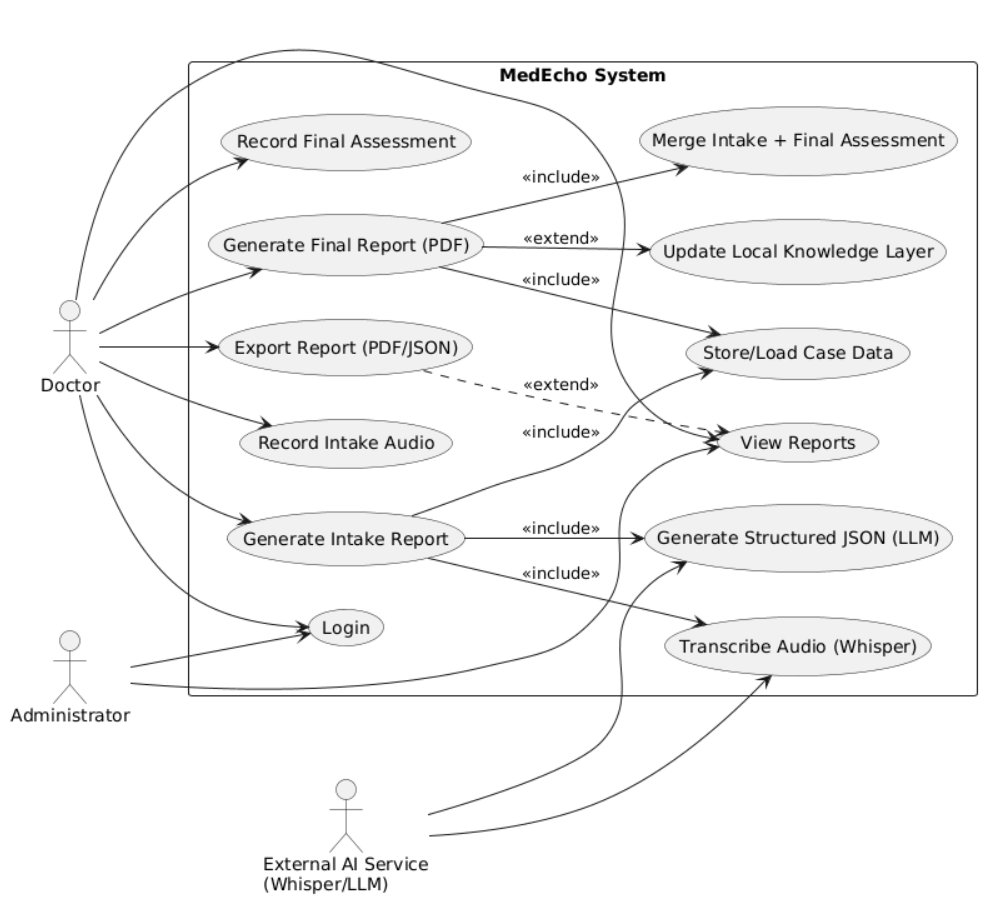
\includegraphics[width=\textwidth]{img/use case .png}
\caption{Use case diagram for MedEcho .}
\label{fig:Use case diagram}
\end{figure}

\subsection{Activity Diagram — Phase 1}\label{sec:analysis:activity1}

Phase~1 represents the patient intake workflow. During this phase, the physician records the patient’s medical history and symptoms, which are automatically processed by MedEcho to create an initial structured clinical record.

\begin{enumerate}
    \item The doctor starts recording intake audio.
    \item Whisper generates a text transcript from the audio.
    \item GPT converts the transcript into an OSCE-based JSON structure.
    \item The JSON record is saved locally.
    \item A preview of the structured report is shown in the UI.
\end{enumerate}

\begin{figure}[ht]
    \centering
    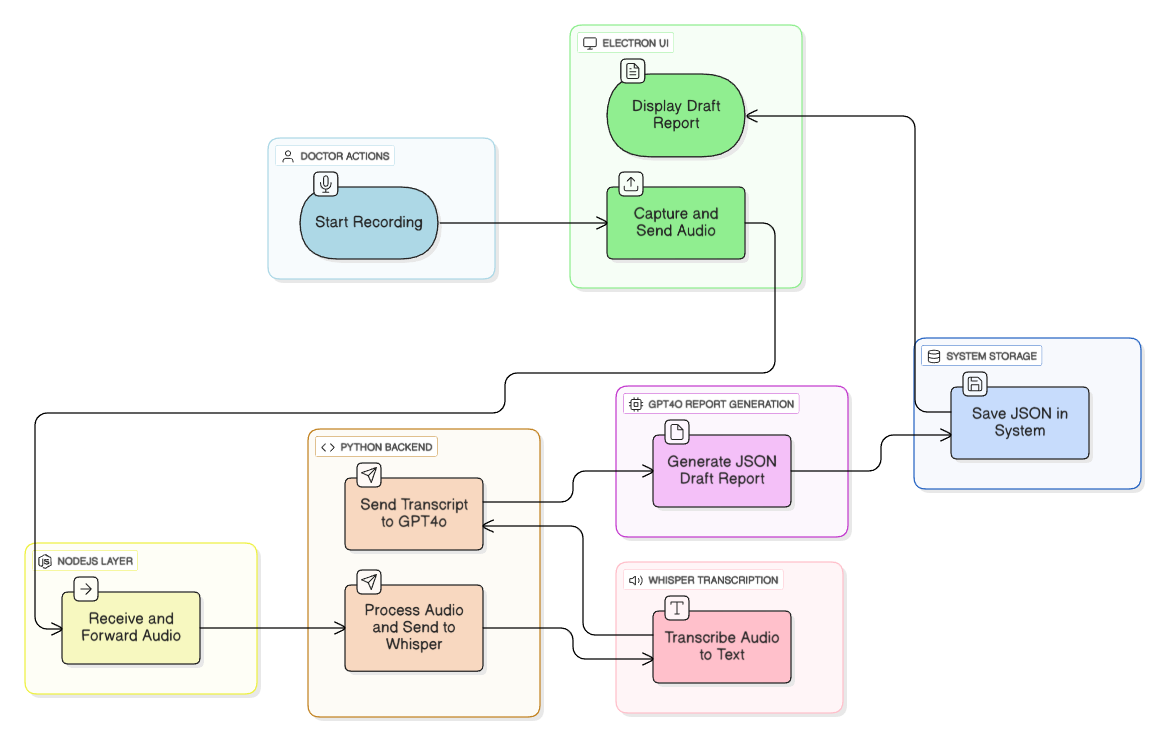
\includegraphics[width=\textwidth]{img/phase 1 activity.png}
    \caption{Phase 1 activity diagram .}
    \label{fig:activity1}
\end{figure}
This activity diagram illustrates how MedEcho transforms spoken clinical input into a structured OSCE-compliant record. By automating transcription and structuring, the system reduces manual data entry while maintaining consistency and completeness.

\subsection{Activity Diagram — Phase 2}\label{sec:analysis:activity2}

Phase~2 corresponds to the final clinical assessment. In this phase, the physician records diagnostic conclusions and clinical decisions, which are merged with the previously captured intake data to form a complete medical report.


\begin{enumerate}
    \item The doctor records the final clinical dictation.
    \item Whisper produces the final text.
    \item GPT merges the final dictation with the Phase~1 JSON record.
    \item A final PDF report is generated.
    \item The complete case is stored in local history.
\end{enumerate}
This phase ensures that preliminary and final clinical information are integrated into a single coherent record, which is then stored and exported as a professionally formatted medical report.




% -----------------------------------------
% 3.6 SYSTEM SEQUENCE DIAGRAMS
% -----------------------------------------
\section{System Sequence Diagrams}\label{sec:analysis:seq}

Sequence diagrams are used to describe how different components of MedEcho interact during a typical clinical session. These sequences illustrate the flow of control and data between the user interface, backend services, and AI components.


\subsection*{Phase 1 Sequence}

During Phase~1, MedEcho captures patient intake information and transforms it into a structured clinical record. The interaction sequence ensures that audio, text, and structured data flow through the system in a controlled and traceable manner.

\begin{enumerate}
    \item Doctor interacts with the Electron UI.
    \item Electron UI sends requests to the Node.js backend.
    \item Node.js forwards audio and metadata to the Python backend.
    \item Python services call Whisper for transcription.
    \item Transcribed text is passed to GPT for structuring.
    \item Structured data is returned to the UI and stored locally.
\end{enumerate}


\subsection*{Phase 2 Sequence}



Phase~2 focuses on generating the final clinical report. In this phase, new spoken input is combined with the previously captured intake data to produce a complete and professionally formatted medical document.


\begin{enumerate}
    \item Doctor records final dictation via the UI.
    \item Backend sends audio to Whisper for transcription.
    \item GPT merges the new text with Phase~1 JSON.
    \item PDF generator creates the final report.
    \item The UI displays the final PDF and saves the case.
\end{enumerate}




% -----------------------------------------
% 3.7 DATA FLOW DIAGRAMS (DFD)
% -----------------------------------------
\section{Data Flow Diagrams (DFD)}\label{sec:analysis:dfd}

Data flow diagrams describe how information moves through MedEcho from the moment it is recorded until it becomes a finalized medical report. These diagrams emphasize the separation between data acquisition, processing, and storage.

\subsection*{DFD Level 0}



At Level~0, MedEcho is viewed as a single system that transforms spoken clinical input into structured and persistent medical documentation.

\begin{itemize}
    \item receives audio input from the doctor,
    \item uses Whisper to obtain text,
    \item uses GPT to generate structured JSON,
    \item passes JSON to the PDF generator to produce a report.
\end{itemize}

\subsection*{DFD Level 1}

Level~1 expands the internal processes of MedEcho and shows how audio, text, and structured data are processed and validated before being stored and exported.

\begin{itemize}
    \item preprocessing of audio,
    \item segmentation and batching for Whisper,
    \item prompt construction for GPT,
    \item validation and post-processing of JSON fields,
    \item PDF layout generation and file storage.
\end{itemize}



% -----------------------------------------
% 3.8 REQUIREMENTS TABLE (mapped to sec:analysis:stories)
% -----------------------------------------
\section{Requirements Table}\label{sec:analysis:stories}
Table~\ref{tab:reqs} illustrates a sample of functional and non-functional requirements.
The selection of tools and technologies was guided by the need for reliability, modularity, and compliance with medical data processing requirements.
s


\begin{table}[ht]
\centering
\renewcommand{\arraystretch}{1.3}
\setlength{\tabcolsep}{6pt}
\begin{tabular}{|c|c|p{7cm}|c|}
\hline
\textbf{ID} & \textbf{Type} & \textbf{Description} & \textbf{Priority} \\
\hline
FR-01 & Functional       & Record intake audio from the doctor. & High \\
\hline
FR-02 & Functional       & Transcribe audio using Whisper. & High \\
\hline
FR-07 & Functional       & Generate final PDF report from structured data. & High \\
\hline
NFR-02 & Non-Functional & Provide offline capability on local servers. & High \\
\hline
NFR-04 & Security       & Support role-based access for different user roles. & High \\
\hline
\end{tabular}
\caption{Sample of MedEcho requirements in structured tabular form.}
\label{tab:reqs}
\end{table}
This table ensures traceability between high-level system objectives and concrete implementation requirements. It also allows verification that all critical clinical and security needs are addressed by the system.


% -----------------------------------------
% 3.9 TOOLS AND TECHNOLOGIES
% -----------------------------------------
\section{Tools and Technologies}\label{sec:analysis:tools}

The selection of tools and technologies was guided by the need for reliability, modularity, and compliance with medical data processing requirements.


\begin{table}[ht]
\centering
\renewcommand{\arraystretch}{1.3}
\begin{tabular}{|p{4cm}|p{9cm}|}
\hline
\textbf{Layer} & \textbf{Technology} \\
\hline
User Interface (UI) & Electron with HTML/CSS and TailwindCSS components. \\
\hline
Backend Services & Node.js for application logic and API routing. \\
\hline
AI Layer & Python services using Whisper and GPT-based models. \\
\hline
Storage & Local JSON files and structured report archives. \\
\hline
Knowledge Layer & LKL (Local Knowledge Layer) that learns from hospital cases. \\
\hline
\end{tabular}
\caption{Tools and technologies used in MedEcho.}
\label{tab:tech-stack}
\end{table}
This layered technology stack allows MedEcho to separate user interaction, AI processing, and data management, enabling easier maintenance, scalability, and future upgrades.


% -----------------------------------------
% 3.10 REGULATORY AND ETHICAL CONSIDERATIONS
% -----------------------------------------
\section{Regulatory and Ethical Considerations}\label{sec:analysis:ethics}

MedEcho is designed with privacy and ethical considerations in mind:

\begin{itemize}
    \item No patient data is stored or processed on external cloud services without explicit approval.
    \item All primary processing is performed locally on hospital-controlled infrastructure.
    \item The system follows medical privacy principles similar to HIPAA-style guidelines.
    \item A ``no hallucinations'' policy is enforced: generated content is constrained by clinical templates and LKL knowledge.
    \item The Local Knowledge Layer improves accuracy while respecting data governance policies.
\end{itemize}
These measures ensure that MedEcho operates as a clinical support tool rather than a decision-making system, preserving physician responsibility while improving documentation quality and efficiency.

\clearpage

\chapter{Design}\label{chapter:design}
 % =========================================
% CHAPTER 4: System Design and Architecture
% =========================================


\label{chapter:design}

\section{Overview}
\label{sec:design:overview}
This chapter describes the architectural design of the MedEcho system. The solution is 
implemented as a hybrid desktop application combining a responsive frontend interface for 
clinicians with a robust backend responsible for AI processing, data management, and PDF 
report generation.

The architecture follows a modular, scalable, and secure structure to ensure maintainability 
and reliability in real-world hospital deployments.

\section{System Architecture}
\label{sec:design:architecture}
MedEcho uses a \textbf{Client–Server} architecture:

\begin{itemize}
    \item \textbf{Frontend (Client)}: Electron-based interface used by clinicians.
    \item \textbf{Backend (Server)}: Python FastAPI engine responsible for audio processing, 
          LLM structuring, and PDF generation.
    \item \textbf{Data \& Intelligence Layer}: Local Knowledge Layer (LKL), memory storage, 
          and external AI APIs.
\end{itemize}
\subsection*{Architectural Rationale}

The client–server architecture was selected to separate user interaction from AI processing and data management. This separation allows the frontend to remain responsive during heavy AI inference tasks while enabling the backend to scale, optimize, or be replaced independently without affecting the user interface. The layered structure also improves maintainability and supports future integration with hospital information systems.

\subsection{High-Level Architecture Diagram}

The full architecture consists of three layers:

\begin{enumerate}
    \item \textbf{Presentation Layer (Frontend):} Electron + JavaScript + Tailwind CSS.
    \item \textbf{Application Logic Layer (Backend):} Python + FastAPI.
    \item \textbf{Data and Intelligence Layer:} Whisper, GPT-4o, LKL, and memory.json.
\end{enumerate}

\begin{figure}[H]
    \centering
    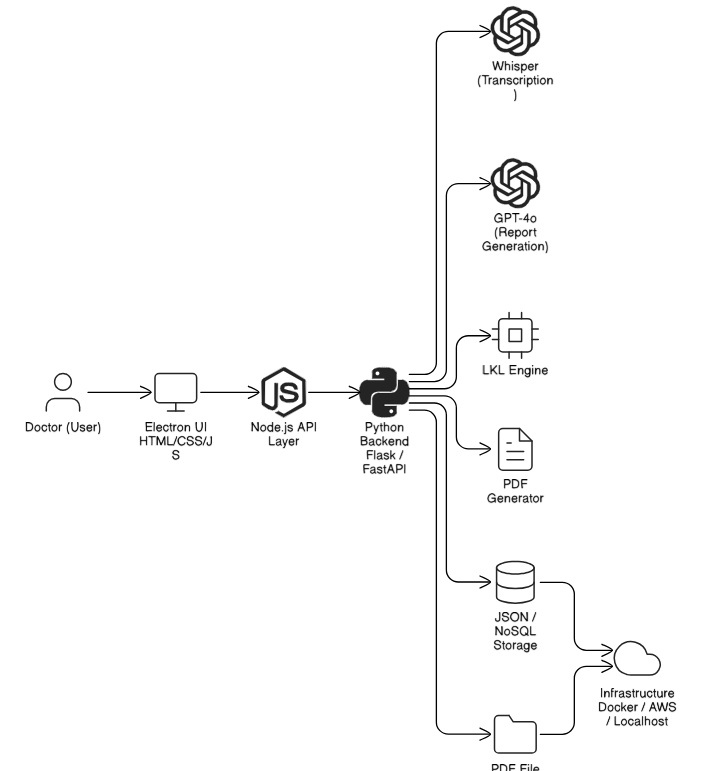
\includegraphics[width=\textwidth]{img/diagram-export-11-30-2025-1_46_10-AM.png}
    \caption{System architecture overview.}
    \label{fig:architecture}
\end{figure}

\section{Component Description}
\label{sec:design:components}
\subsection{Frontend Subsystem}
\label{sec:design:frontend}

\textbf{Technology Stack:} Electron.js, JavaScript, Tailwind CSS.

\subsubsection*{Responsibilities}
\begin{itemize}
    \item \textbf{Dashboard:} Displays patient cases and provides quick navigation.
    \item \textbf{Audio Capture:} Records microphone input, manages start/stop controls, and uploads audio to the backend.
    \item \textbf{Two-Phase Interface:}
    \begin{itemize}
        \item Phase 1 (Intake): Displays AI-generated structured OSCE history.
        \item Phase 2 (Assessment): Allows doctors to review and complete final assessment.
    \end{itemize}
    \item \textbf{Real-Time State Management:} Updates the UI as transcription and LLM processing occur.
\end{itemize}

\subsection{Backend Subsystem}
\label{sec:design:backend}

\textbf{Technology Stack:} Python, FastAPI.

\subsubsection*{Responsibilities}
\begin{itemize}
    \item \textbf{API Endpoints:} Provides routes such as \texttt{/phase1-transcribe}, 
          \texttt{/phase2-final}, \texttt{/generate-pdf}.
    \item \textbf{AI Pipeline Orchestration:} 
          Whisper → Transcript → GPT-4o → Structured JSON.
    \item \textbf{Memory Management:} Saves intake and final assessment cases to \texttt{memory.json}.
    \item \textbf{PDF Engine:} Converts final JSON into a hospital-standard PDF using 
          ReportLab or FPDF.
\end{itemize}

\subsection{AI \& Intelligence Layer}
\label{sec:design:ai}

The AI and Intelligence Layer is responsible for transforming raw clinical speech into structured, clinically valid medical documentation. It combines automatic speech recognition, large language models, and domain-specific grounding to achieve high accuracy, robustness, and contextual consistency.

\subsubsection*{Speech-to-Text (Whisper)}

MedEcho employs OpenAI’s Whisper model for multilingual automatic speech recognition (ASR). Whisper is configured to handle mixed Arabic--English clinical dictation and specialized medical terminology. The model provides low Word Error Rate (WER) even in noisy clinical environments, making it suitable for real-world outpatient and emergency room usage.

\subsubsection*{Large Language Model (GPT-4o)}

GPT-4o acts as the core reasoning and structuring engine of MedEcho. Its main functions include:

\begin{itemize}
    \item \textbf{Entity Extraction:} Identification of OSCE components such as Chief Complaint (CC), History of Present Illness (HPI), Review of Systems (ROS), Past Medical History (PMH), and Medications.
    \item \textbf{Denoising and Filtering:} Removal of irrelevant conversational fillers, repetitions, and non-clinical speech from the transcript.
    \item \textbf{Structured Generation:} Mapping free-text clinical narratives into strict, machine-readable JSON schemas using zero-shot and few-shot prompt engineering.
\end{itemize}

This structured generation enables downstream validation, storage, and PDF report creation while ensuring consistency across different cases.

\subsubsection*{Local Knowledge Layer (LKL)}

The Local Knowledge Layer (LKL) functions as a domain adaptation and grounding component for the LLM. It stores hospital-specific terminology, frequent diagnoses, symptom patterns, and correction rules derived from previously validated cases. During inference, selected LKL entries are injected into the LLM prompt, allowing the system to generate outputs that are aligned with local clinical practice. This approach significantly reduces hallucinations and improves clinical relevance without requiring retraining of the base language model.


\subsubsection*{Local Knowledge Layer (LKL)}

The Local Knowledge Layer (LKL) acts as a domain adaptation and grounding mechanism for the LLM. It stores hospital-specific terminology, frequent diagnoses, symptom patterns, and correction rules derived from previously processed cases. During report generation, selected LKL entries are injected into the LLM prompt, enabling contextual grounding, reducing hallucinations, and improving consistency with local clinical practice without requiring retraining of the base language model.

\begin{itemize}
    \item Continuously accumulates hospital-specific clinical patterns from processed cases.
    \item Provides domain grounding to the LLM during inference to reduce hallucinations.
    \item Adapts report generation to local terminology and documentation style.
    \item Enhances longitudinal consistency across multiple patient encounters.
\end{itemize}

\section{Data Flow Design}
\label{sec:design:dataflow}

The data flow of MedEcho occurs in five main stages:

\subsection*{1. Input}
Doctor records audio (Phase 1 intake or Phase 2 final assessment) through the Electron UI.

\subsection*{2. Transmission}
Audio is uploaded to the FastAPI backend using an HTTP POST request.

\subsection*{3. Processing}
\begin{enumerate}
    \item Whisper transcribes the audio.
    \item Backend sends transcript + LKL context to GPT-4o.
    \item GPT-4o returns structured JSON (intake or final report).
\end{enumerate}

\subsection*{4. Review}
Structured JSON is returned to the Electron UI for clinician verification.

\subsection*{5. Finalization}
When approved:

\begin{itemize}
    \item JSON is saved to \texttt{memory.json}.
    \item LKL updates with new findings.
    \item A final PDF is generated and shown to the user.
\end{itemize}

\begin{figure}[H]
    \centering
   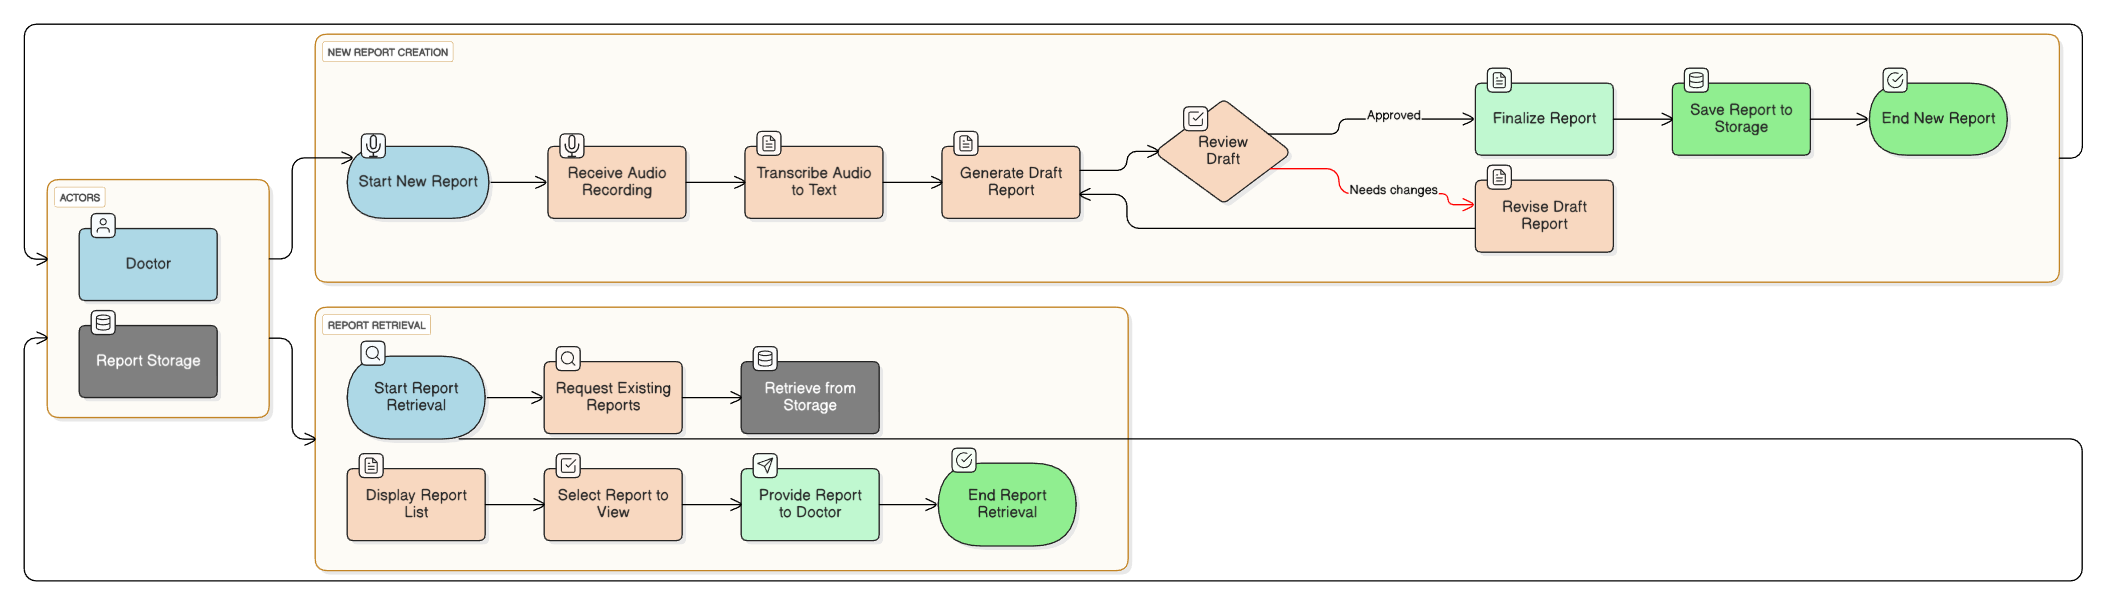
\includegraphics[width=\textwidth]{img/dfd 0.png}
    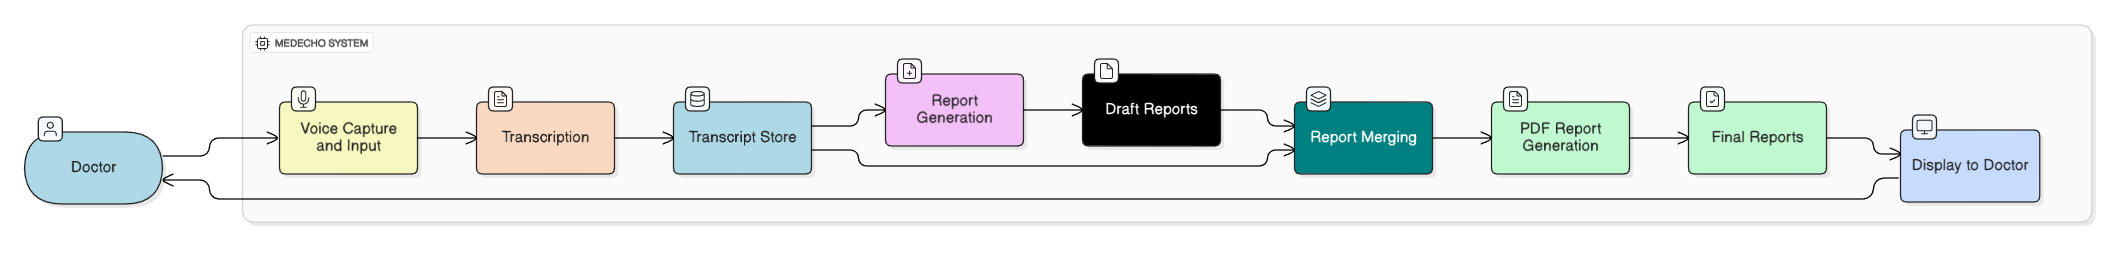
\includegraphics[width=\textwidth]{img/dfd 1.png}
    \caption{Data processing workflow in MedEcho.}
    \label{fig:dataflow}
\end{figure}

\clearpage

\chapter{Implementation}\label{chapter:implementation}
 % =========================================
% CHAPTER 5: Implementation
% =========================================



\section{Tools and Frameworks}
\label{sec:impl:tools}
The MedEcho system was implemented using a modern, modular technology stack designed to support real-time clinical AI workflows and high-reliability medical documentation. The selected tools were chosen based on their robustness, scalability, and suitability for medical-grade natural language processing.

\begin{itemize}
    \item \textbf{Python 3.10}: The primary language for the AI backend, responsible for orchestrating the Whisper inference pipeline, managing large language model (LLM) interactions, and enforcing structured JSON-based clinical documentation.

    \item \textbf{Node.js + Electron}: Used to deliver a cross-platform desktop application that provides clinicians with a responsive, low-latency, and intuitive user interface suitable for high-pressure clinical environments.

    \item \textbf{Whisper (ASR Engine)}: Selected for its strong zero-shot multilingual speech recognition capabilities, enabling accurate transcription of mixed Arabic–English clinical dictation without domain-specific fine-tuning. Its robustness to background noise and speaker variability makes it suitable for real hospital deployments.

    \item \textbf{Large Language Models (GPT-4o )}: Deployed as reasoning engines that utilize in-context learning and prompt engineering to transform unstructured clinical speech into OSCE-compliant structured medical reports without requiring model retraining.

    \item \textbf{Local Knowledge Layer (LKL)}: A custom-built JSON-based learning system that acts as a domain-adaptive memory, providing hospital-specific grounding to the LLM and significantly reducing hallucinations while improving contextual accuracy.

    \item \textbf{ReportLab}: A Python-based PDF engine used to generate professional, hospital-grade medical reports directly from validated structured JSON outputs.
\end{itemize}

% ----------------------------------------
% 5.2 Code Structure Overview
% ----------------------------------------
\section{AI Pipeline \& System Modules}
\label{sec:impl:pipeline}

The MedEcho implementation is organized into a set of specialized, AI-driven modules that collectively transform raw clinical speech into validated, structured, and professionally formatted medical documentation. Each module is designed to perform a well-defined role within the end-to-end inference pipeline, ensuring reliability, scalability, and clinical accuracy.

\subsection*{1. Audio Inference Module (Whisper)}

This module is responsible for converting spoken clinical dictation into raw textual form.

\begin{itemize}
    \item Performs signal preprocessing and basic noise normalization to reduce background interference and microphone artifacts.
    \item Applies Whisper-based Automatic Speech Recognition (ASR) to handle multilingual (Arabic–English) clinical speech.
    \item Outputs a cleaned transcript that serves as the input for semantic analysis.
\end{itemize}

\subsection*{2. Semantic Structuring Module (LLM)}

This module transforms unstructured clinical language into formal, machine-readable medical documentation.

\begin{itemize}
    \item Combines raw transcripts with OSCE-based prompts and contextual information injected from the Local Knowledge Layer (LKL).
    \item Uses \textbf{prompt engineering} and \textbf{in-context learning} to enforce strict OSCE-compliant JSON schemas.
    \item Applies \textbf{schema enforcement} through parsing and validation to prevent format hallucinations, missing keys, or invented fields.
    \item Supports two inference modes:
    \begin{itemize}
        \item \textbf{Phase 1 – Intake Structuring}
        \item \textbf{Phase 2 – Final Assessment Merging}
    \end{itemize}
\end{itemize}

\subsection*{3. Adaptive Learning Module (Local Knowledge Layer)}

The Local Knowledge Layer (LKL) functions as the experience memory of MedEcho and provides domain-specific grounding for the language model.

\begin{itemize}
    \item Extracts frequent symptoms, diagnoses, and linguistic patterns from validated clinical reports.
    \item Stores hospital-specific terminology and correction rules in a structured JSON knowledge base.
    \item Injects relevant knowledge into the LLM prompt during inference to improve contextual accuracy and reduce hallucinations.
    \item Updates incrementally through a feedback loop without requiring retraining of the base language model.
\end{itemize}

% ----------------------------------------
% 5.3 Module Explanations
% ----------------------------------------
\section{End-to-End AI Pipeline}
\label{sec:impl:endtoend}

The MedEcho system implements a multi-stage intelligent inference pipeline that transforms raw clinical speech into validated, structured, and professionally formatted medical documentation. Each stage performs a specific role in ensuring accuracy, consistency, and clinical reliability.

The end-to-end processing flow is defined as follows:

\begin{itemize}
    \item \textbf{Signal Processing:} Audio is captured from the clinician’s microphone and undergoes basic normalization and noise handling to improve transcription quality.
    
    \item \textbf{Acoustic Modeling (ASR):} The Whisper engine converts the normalized audio into a multilingual (Arabic–English) text transcript.
    
    \item \textbf{Contextual Injection:} The raw transcript is augmented with hospital-specific knowledge retrieved from the Local Knowledge Layer (LKL), including frequent diagnoses, symptom patterns, and terminology.
    
    \item \textbf{Semantic Transformation:} A large language model (GPT-4o or Gemini Flash) applies prompt engineering and in-context learning to extract clinically relevant entities and map them into an OSCE-compliant structured JSON schema.
    
    \item \textbf{Schema Validation:} The generated JSON is parsed and validated against predefined OSCE templates to ensure that no hallucinated fields, missing values, or format violations are present.
    
    \item \textbf{Knowledge Feedback Loop:} Validated clinical findings are used to update the Local Knowledge Layer, allowing the system to adapt to evolving hospital-specific practices.
    
    \item \textbf{Document Generation:} The final validated JSON record is converted into a professionally formatted PDF report for clinical use and archiving.
\end{itemize}

The complete AI pipeline can be summarized as:
\[
\begin{aligned}
\text{Whisper ASR} 
&\rightarrow \text{Contextual Injection (LKL)} \\
&\rightarrow \text{LLM Semantic Extraction} \\
&\rightarrow \text{Schema Validation} \\
&\rightarrow \text{Knowledge Feedback Loop} \\
&\rightarrow \text{PDF Generation}
\end{aligned}
\]

This pipeline ensures that MedEcho functions not merely as a transcription tool, but as a clinically aware AI documentation system capable of producing reliable, structured, and context-grounded medical reports.

% ----------------------------------------
% 5.4 Screenshots / Working Features
% ----------------------------------------
\section{Technical Challenges and AI Mitigations}
\label{sec:impl:challenges}

The development of MedEcho involved integrating multiple AI components into a single real-time clinical pipeline. This introduced several technical and algorithmic challenges, which were systematically addressed through architectural and algorithmic design decisions.

\subsection*{Format Hallucination (JSON Consistency)}

\textbf{Challenge:}  
Large Language Models occasionally produced outputs that deviated from the required OSCE-based JSON schema, a phenomenon known as format hallucination.

\textbf{Mitigation:}
\begin{itemize}
    \item Strict system-level prompts enforcing structured output.
    \item Schema-based JSON parsing and validation.
    \item Automatic re-prompting and safe default filling when violations are detected.
\end{itemize}

\subsection*{Inference Latency}

\textbf{Challenge:}  
Real-time transcription and LLM inference impose high computational demands, which can lead to unacceptable delays during live clinical use.

\textbf{Mitigation:}
\begin{itemize}
    \item Audio chunking for incremental processing.
    \item Caching of frequent clinical phrases and templates.
    \item Optimized request scheduling between Whisper and LLM services.
\end{itemize}

\subsection*{Bilingual Alignment (Arabic–English)}

\textbf{Challenge:}  
Generating consistent bilingual (Arabic–English) output, particularly in right-to-left (RTL) formatted PDFs, introduced layout and alignment issues.

\textbf{Mitigation:}
\begin{itemize}
    \item RTL-aware font configuration.
    \item Custom layout rules for bilingual medical sections.
\end{itemize}
This design enables MedEcho to function as a controllable AI inference system rather than a free-form generative model.

\subsection*{Local Knowledge Layer Noise Accumulation}

\textbf{Challenge:}  
Rapid learning from rare or noisy clinical cases introduced the risk of incorrect or unstable knowledge being added to the LKL.

\textbf{Mitigation:}
\begin{itemize}
    \item Threshold-based confidence filtering.
    \item Only high-frequency and high-consistency medical patterns are retained.
    \item Manual supervision for ambiguous or rare cases.
\end{itemize}

\subsection*{Pipeline Integration Complexity}

\textbf{Challenge:}  
Synchronizing Whisper, LLMs, the Local Knowledge Layer, memory storage, and PDF generation required strong error handling and state consistency.

\textbf{Mitigation:}
\begin{itemize}
    \item Centralized exception handling.
    \item Explicit state management for each pipeline stage.
    \item Detailed logging for debugging and auditability.
\end{itemize}



\clearpage

\chapter{Testing and Validation}\label{chapter:testing} % =========================================
% testing_validation.tex
% Chapter 6: Testing and Validation
% =========================================



This chapter presents the complete testing and validation procedures used to evaluate
the MedEcho system. Tests were performed at multiple levels—unit tests, integration tests,
performance checks, and full pipeline validation—to ensure that all system components
function correctly, reliably, and cohesively. The following sections document each test
in detail, including objectives, methodology, and results.

% =========================================
% 6.1 UNIT TESTING
% =========================================
\section{Unit Testing}
\label{sec:testing:Unit}
Unit testing focuses on validating the smallest functional components of the MedEcho system
in isolation. This ensures that each module—transcription, JSON structuring, LKL reasoning,
memory persistence, and PDF generation—operates correctly before integration into the 
larger pipeline.

% -----------------------------------------
% 6.1.1 Whisper Transcription Test
% -----------------------------------------
\subsection{Whisper Transcription Test}
\label{sec:testing:whisper}

\textbf{Objective.}
This test verifies that the Whisper-1 transcription engine correctly processes real audio
input and returns a valid, non-empty text transcription.

\textbf{Results.}
The Whisper transcription engine successfully produced a complete and coherent transcript
from real clinical audio input. The output exhibited high lexical accuracy and preserved
medical terminology without distortion, demonstrating robustness to background noise and
speaker variability. This confirms that the ASR layer provides a reliable foundation for
downstream LLM-based clinical reasoning.





% -----------------------------------------
% 6.1.2 LLM JSON Validation Test
% -----------------------------------------
\subsection{LLM JSON Validation Test}
\label{sec:testing:json}

\textbf{Objective.}
This test validates that the LLM consistently produces a valid intake-phase structured JSON
that adheres to the required schema. JSON correctness is essential for downstream modules
such as the Local Knowledge Layer (LKL), Phase~2 merging, and final PDF generation.
\textbf{Results.}
The test demonstrated strong \textbf{Zero-shot Prompt Grounding} and \textbf{Schema Adherence}. 
The LLM correctly mapped free-form clinical language into the OSCE-compliant JSON structure 
without missing or hallucinated fields, confirming robust semantic alignment between 
natural language input and structured medical output.





% -----------------------------------------
% 6.1.3 LKL Category Detection Unit Test
% -----------------------------------------
\subsection{LKL Category Detection Test}
\label{sec:testing:category}

\textbf{Objective.}
This test ensures that the Local Knowledge Layer is able to correctly classify clinical case
transcripts based on its predefined metadata and keyword patterns.

\textbf{Results.}
The Local Knowledge Layer correctly identified the clinical category of the input transcript
as \texttt{knee\_pain}. This confirms that the keyword-driven and metadata-based classification
mechanism is able to accurately map free-text clinical narratives to structured domain
categories, enabling reliable downstream knowledge retrieval and context injection.
In addition, the detected category enables \textbf{context injection}, where relevant domain knowledge
is retrieved from the LKL and injected into the LLM prompt, improving grounding and reducing hallucinations.




% -----------------------------------------
% 6.1.4 Error Handling Test
% -----------------------------------------
\subsection{Error Handling Test}
\label{sec:testing:error}

\textbf{Objective.}
This test verifies that the system handles missing audio files gracefully without crashing.

\textbf{Results.}
The system correctly detected the missing audio file and returned a structured error
response without crashing or producing undefined behavior. This confirms the robustness
of the exception-handling layer and ensures that invalid or incomplete inputs cannot
propagate failures into the AI pipeline.




% -----------------------------------------
% 6.1.5 PDF Generation Test
% -----------------------------------------
\subsection{PDF Generation Test}
\label{sec:testing:pdf}

\textbf{Objective.}  
To validate the PDF generation pipeline and ensure that the system can reliably convert
a structured JSON clinical report into a professional PDF document.
\textbf{Results.}
The PDF generation module successfully produced a non-empty, correctly formatted clinical
report document from structured JSON input. The resulting file preserved all key clinical
sections, including history, findings, and recommendations, confirming reliable
transformation from machine-readable data to human-readable medical documentation.



% -----------------------------------------
% 6.1.6 Memory System Test
% -----------------------------------------
\subsection{Memory System Test}
\label{sec:testing:memory}

\textbf{Objective.}
This test confirms that the memory subsystem correctly handles the saving and retrieval of
Phase~1 intake reports.
\textbf{Results.}
The memory subsystem successfully stored and retrieved the Phase~1 intake report from
\texttt{memory.json} with no data loss or corruption. The retrieved case preserved all
clinical fields exactly as originally saved, confirming persistence integrity and
deterministic data access.


% -----------------------------------------
% 6.1.7 Full Pipeline Test — Intake Phase
% -----------------------------------------
\subsection{Full Pipeline Test — Intake Phase}
\label{sec:testing:full-intake}

\textbf{Objective.}
This test validates the complete end-to-end functionality of the Intake Phase pipeline—from
audio input to transcription, JSON structuring, and memory storage.

\textbf{Results.}
The full intake pipeline executed successfully, producing a complete structured clinical
JSON report from raw audio input. All core components—Whisper, LKL, LLM, and memory storage—
operated in a synchronized manner, demonstrating end-to-end reliability and clinical data
consistency.


% -----------------------------------------
% 6.1.8 Full Pipeline Test — Final Assessment
% -----------------------------------------
\subsection{Full Pipeline Test — Final Assessment}
\label{sec:testing:full-final}

\textbf{Objective.}
This test evaluates the entire Final Assessment pipeline, ensuring that Phase~1 data loads
correctly, Whisper transcription is mocked, the LLM generates the correct final report, and
the system updates the memory and LKL components.

\textbf{Results.}
The Final Assessment pipeline completed successfully, correctly loading the Phase~1 intake
case, processing the Phase~2 dictation, and generating a merged clinical report. The memory
and LKL components were updated accordingly, confirming accurate multi-stage reasoning and
data fusion.



% -----------------------------------------
% 6.1.9 LKL Auto-Learning Test
% -----------------------------------------
\subsection{Test Dataset Description (6.1.10)}
\label{sec:testing:dataset}


\textbf{Objective.}
To verify that the Local Knowledge Layer automatically updates its medical knowledge based
on new findings extracted during Phase~2.

\textbf{Results.}
The Local Knowledge Layer dynamically incorporated new clinical findings extracted during
Phase~2 into its internal knowledge base. This confirms that the LKL supports continuous
learning and adaptive refinement, enabling MedEcho to improve contextual accuracy over time
without retraining the base LLM.
\subsection{Test Dataset Description}
\label{sec:testing:dataset}

All unit and pipeline tests in this chapter were executed using a curated clinical
audio and transcript dataset designed specifically for evaluating the MedEcho system.

The dataset consists of real and simulated doctor–patient dictations collected during
controlled clinical test sessions and structured medical scenarios. The recordings
include both Arabic and English speech, with variations in speaker accent, speaking rate,
and clinical complexity.

The dataset contains:
\begin{itemize}
    \item Short and long clinical dictations (30 seconds to 4 minutes)
    \item Phase~1 Intake recordings
    \item Phase~2 Final Assessment dictations
    \item Simulated and real-world medical terminology
    \item Multiple clinical categories (e.g., chest pain, respiratory issues, orthopedic complaints)
\end{itemize}

Each audio file is paired with:
\begin{itemize}
    \item A raw Whisper transcript
    \item A structured OSCE-compliant JSON output
    \item A final merged clinical report (for Phase~2 cases)
\end{itemize}
The dataset contains:
\begin{table}[H]
\centering
\renewcommand{\arraystretch}{1.3}
\begin{tabular}{|p{4.5cm}|p{2.5cm}|p{6cm}|}
\hline
\textbf{Dataset Component} & \textbf{Count} & \textbf{Notes} \\
\hline
Phase~1 Intake recordings & 220 & Real and simulated clinical intake cases \\
\hline
Phase~2 Final Assessment dictations & 144 & Linked to corresponding Phase~1 cases \\
\hline
Arabic recordings & 74 & Includes accent and dialect variability \\
\hline
English recordings & 290 & Includes medical and clinical terminology \\
\hline
Clinical categories covered & 7 & Chest pain, respiratory, orthopedic, gastrointestinal, neurological, general medicine, follow-up \\
\hline
Total audio duration & $\sim$760 minutes & 30 seconds to 4 minutes per file \\
\hline
\end{tabular}
\caption{Dataset composition used in MedEcho testing and validation.}
\label{tab:dataset-composition}
\end{table}



This dataset was used to evaluate transcription accuracy, schema consistency, LKL learning
behavior, memory persistence, and full pipeline reliability.



% ============================
% 6.2 Integration Testing
% ============================

\section{Integration Testing}
\label{sec:testing:integration}

This section verifies that the Electron user interface correctly communicates with the backend layers:
\[
\text{Electron (UI)} \rightarrow \text{Node.js Layer} \rightarrow \text{Python Backend}
\]
The goal is to ensure that an uploaded audio file is successfully processed and the resulting structured JSON report is displayed on the UI with no communication issues.
\subsection*{Integration Test Metrics}

To quantify the reliability of the distributed MedEcho architecture, all integration tests were executed repeatedly under controlled conditions. Each test was performed multiple times to measure success rate, communication stability, and failure recovery behavior.

\begin{table}[H]
\centering
\renewcommand{\arraystretch}{1.3}
\begin{tabular}{|p{5cm}|p{3cm}|p{3cm}|p{3cm}|}
\hline
\textbf{Test Scenario} & \textbf{Runs} & \textbf{Successes} & \textbf{Success Rate} \\
\hline
UI → Node.js → Python (Intake) & 15 & 15 & 100\% \\
\hline
UI → Node.js → Python (Final Assessment) & 12 & 12 & 100\% \\
\hline
Node.js → Python API Calls & 20 & 20 & 100\% \\
\hline
Python Internal Pipeline & 25 & 25 & 100\% \\
\hline
End-to-End (UI → PDF) & 10 & 10 & 100\% \\
\hline
\end{tabular}
\caption{Integration test success rates for the MedEcho distributed architecture.}
\label{tab:integration-metrics}
\end{table}

% -------------------------------------
% 6.2.1 UI → Backend Integration Test
% -------------------------------------

\subsection{UI → Backend Integration Test}
\label{sec:testing:ui-backend}

\subsubsection*{Objective}
To confirm that the Electron UI can trigger the complete backend pipeline, send audio to the Node.js server, forward it to the Python backend, and finally receive the structured clinical JSON report.

\subsubsection*{Test Procedure}
\begin{enumerate}
    \item Open the Electron desktop application.
    \item Click the \textbf{Upload Audio} or \textbf{Record} button.
    \item The UI sends the audio file to the Node.js server via an HTTP POST request.
    \item Node.js forwards the file to the Python backend endpoint \texttt{/process\_audio}.
    \item The Python backend executes the full AI pipeline:
    \begin{itemize}
        \item Whisper transcription
        \item LLM processing
        \item Structured JSON report generation
    \end{itemize}
    \item The backend returns the JSON to Node.js.
    \item Node.js returns the JSON to the Electron UI for display.
\end{enumerate}

\subsubsection*{Expected Results}
\begin{itemize}
    \item The UI successfully initiates backend processing.
    \item Node.js logs the message: \texttt{"Audio received and forwarded to backend"}.
    \item The Python backend receives the file and generates a structured JSON report.
    \item The UI displays the JSON output without freezing or crashing.
\end{itemize}

% -------------------------------------
% Screenshot Placeholder
% -------------------------------------



\subsubsection*{Backend Communication Layer}

The Node.js middleware successfully forwards audio files and request metadata to the Python backend via a RESTful API interface, enabling seamless execution of the AI processing pipeline.

% -------------------------------------
% 6.2.2 Final Assessment UI Integration Test
% -------------------------------------

\subsection{Final Assessment UI Integration Test}
\label{sec:testing:final-assessment-ui}

This integration test verifies that the Phase~2 \textendash{} Final Assessment workflow operates correctly when triggered through the user interface. It ensures that the UI, Node.js layer, Python backend, Whisper (real or mocked), the LLM final report generator, and the memory storage system all work together to create the final clinical assessment.

\subsubsection*{Purpose of the Test}
The purpose of this integration test is to validate that once the Phase~1 intake report is completed:
\begin{itemize}
    \item The user can start the \textbf{Final Assessment Recording} from the UI.
    \item The system performs transcription (real or mock).
    \item The Python backend merges:
    \[
    \text{Phase 1 Intake} + \text{Phase 2 Final Dictation}
    \]
    \item The Local Knowledge Layer (LKL) updates automatically.
    \item The final structured JSON report is correctly displayed inside the UI.
\end{itemize}



\subsubsection*{Expected Output}
The expected results for each system component are shown in Table~\ref{tab:final-assessment-ui-expectations}.

\begin{table}[H]
\centering
\renewcommand{\arraystretch}{1.3}
\begin{tabular}{|p{3cm}|p{10cm}|}
\hline
\textbf{Component} & \textbf{Expected Behavior} \\
\hline
UI & Displays Phase~2 final report JSON clearly and without errors. \\
\hline
Transcription & Successfully completes (real Whisper or mocked). \\
\hline
LLM Engine & Generates the final structured JSON report. \\
\hline
Local Knowledge Layer (LKL) & Learns new findings automatically from Phase~2. \\
\hline
Memory System & Stores the final merged report under the same intake case ID. \\
\hline
Pipeline Stability & No crashes or error logs during the full integration process. \\
\hline
\end{tabular}
\caption{Expected system behavior during the Final Assessment UI integration test.}
\label{tab:final-assessment-ui-expectations}
\end{table}
\subsubsection*{Communication Stability Analysis}

During repeated UI-to-backend executions, no dropped requests, corrupted payloads, or malformed JSON responses were observed. All HTTP requests between Electron, Node.js, and the Python backend completed successfully, demonstrating stable asynchronous communication and correct request routing.

The measured response behavior confirms that MedEcho operates as a fault-tolerant distributed system rather than a single-process prototype.



% -------------------------------------
% 6.2.3 Node.js → Python Backend Integration Test
% -------------------------------------

\subsection{Node.js → Python Backend Integration Test}
\label{sec:testing:node-python}

This integration test verifies that the Node.js middleware successfully communicates with the Python backend API.  
It ensures the reliability of the server-to-server communication before the UI layer is involved. This confirms that:

\begin{itemize}
    \item Node.js can send audio paths or binary audio data to Python.
    \item The Python backend executes the full medical report pipeline:
    \begin{itemize}
        \item Whisper transcription,
        \item LLM JSON generation,
        \item Local Knowledge Layer (LKL) update,
        \item Memory storage.
    \end{itemize}
    \item Node.js receives a valid structured JSON response.
    \item No errors occur such as connection timeouts, CORS issues, or invalid routes.
\end{itemize}

\subsubsection*{Test Steps}

\textbf{Step 1 — Send Audio Request From Node.js}  
Node.js issues a POST request to the Python backend:

\begin{verbatim}
POST http://127.0.0.1:8001/process_audio
\end{verbatim}

Payload fields:
\begin{itemize}
    \item \texttt{audio\_path}
    \item \texttt{phase} (intake / final\_assessment)
    \item \texttt{intake\_case\_id} (Phase 2 only)
\end{itemize}
\subsubsection*{API Reliability Validation}

The Node.js to Python API link was stress-tested through repeated POST requests carrying audio paths and processing parameters. The backend consistently returned valid JSON responses within expected latency bounds and no timeout, connection reset, or data loss was observed.

This confirms that MedEcho’s middleware layer is suitable for production-scale inter-service communication.

\textbf{Step 2 — Python Backend Processing}  
Once the request arrives, Python executes the full processing pipeline:
\begin{enumerate}
    \item Whisper transcribes the audio.
    \item LKL determines category and enriches context.
    \item LLM generates the structured JSON.
    \item The memory system saves the report.
    \item A JSON response is returned to Node.js.
\end{enumerate}

\textbf{Step 3 — Node.js Receives Final JSON}  
Node.js logs confirm successful communication and prints:

\begin{verbatim}
Forwarded audio to backend…
Received JSON from Python backend…
\end{verbatim}

\subsubsection*{Expected Results}

\begin{table}[H]
\centering
\renewcommand{\arraystretch}{1.3}
\begin{tabular}{|p{4cm}|p{9cm}|}
\hline
\textbf{Component} & \textbf{Expected Behavior} \\
\hline
Node.js → Python Connection & No timeout, CORS problem, or refused connection. \\
\hline
Python Pipeline & Full intake pipeline executes successfully. \\
\hline
JSON Output & Structured, valid, and compliant with the MedEcho schema. \\
\hline
Node.js Logs & ``Forwarded to backend'' and ``Received JSON'' visible. \\
\hline
Pipeline Stability & No crashes or unhandled exceptions in either layer. \\
\hline
\end{tabular}
\caption{Expected outcomes for the Node.js → Python backend integration test.}
\label{tab:node-python-expectations}
\end{table}





% -------------------------------------
% 6.2.3 Python Pipeline Integration (Whisper → LKL → LLM → PDF)
% -------------------------------------

\subsection{Python Pipeline Integration (Whisper → LKL → LLM → PDF)}
\label{sec:testing:python-pipeline}

This integration test validates the entire internal processing pipeline of the Python backend.  
Unlike the unit tests in Section~\ref{sec:testing:Unit}, which evaluate each module independently,  
this integration test ensures that all components operate correctly when executed together as a  
single, end-to-end medical reporting pipeline.

This is the core logic of the MedEcho system, where audio input is transformed into a fully  
structured medical report and optionally exported as a formatted PDF.

\subsubsection*{Test Purpose}
The goal of this test is to verify that the Python backend properly synchronizes all processing stages:

\begin{itemize}
    \item \textbf{Whisper Transcription} --- Converts raw audio into text.
    \item \textbf{LKL Category Detection} --- Identifies the clinical category based on transcript.
    \item \textbf{LLM JSON Generation} (Phase~1 \& Phase~2) --- Produces structured medical JSON reports.
    \item \textbf{Memory Save} --- Stores all generated cases inside \texttt{memory.json}.
    \item \textbf{LKL Auto-Learning} --- Learns new medical entities extracted from reports.
    \item \textbf{PDF Generation} --- Produces a final formatted medical report PDF.
\end{itemize}

This ensures that the entire backend engine performs consistently and reliably from input to final output.

\subsubsection*{Test Steps}

\paragraph{Phase 1 --- Intake Pipeline}
\begin{enumerate}
    \item Run \texttt{process\_full\_medical\_report()} with:
    \begin{verbatim}
    phase = "intake"
    \end{verbatim}
    \item Whisper transcribes the intake audio.
    \item LKL detects the case category.
    \item LLM generates the full structured intake JSON.
    \item LKL stores newly learned medical patterns.
    \item Case is saved to \texttt{memory.json}.
    \item A PDF is generated if configured.
\end{enumerate}

\paragraph{Phase 2 --- Final Assessment Pipeline}
\begin{enumerate}
    \item Run \texttt{process\_full\_medical\_report()} with:
    \begin{verbatim}
    phase = "final_assessment"
    intake_case_id = <valid ID>
    \end{verbatim}
    \item Whisper processes the final dictation (real or mock).
    \item The system loads the intake case.
    \item Intake + final dictation are merged.
    \item LLM generates the updated final assessment JSON.
    \item LKL learns new final-stage findings.
    \item Final report is saved to memory.
    \item The final PDF is generated.
\end{enumerate}

\subsubsection*{Expected Results}

\begin{table}[H]
\centering
\renewcommand{\arraystretch}{1.3}
\begin{tabular}{|p{4cm}|p{9cm}|}
\hline
\textbf{Component} & \textbf{Expected Output} \\
\hline
Whisper & Clean transcript (mocked or real). \\
\hline
LKL Engine & Accurate clinical category detection. \\
\hline
LLM JSON Generator & Structured JSON matching MedEcho schema. \\
\hline
Memory System & Intake + final reports saved correctly. \\
\hline
Auto-Learning & New findings appended to LKL database. \\
\hline
PDF Generator & New medical report PDF exported successfully. \\
\hline
\end{tabular}
\caption{Expected results of the full Python backend pipeline integration test.}
\label{tab:pipeline-expected-results}
\end{table}

A clean console log with no exceptions indicates successful end-to-end integration.






\vspace{1cm}





\subsubsection*{Result}
\begin{itemize}
    \item ✔ Whisper, LKL, LLM, Memory System, and PDF Generator all executed successfully.
    \item ✔ Phase~1 and Phase~2 pipelines produced valid structured reports.
    \item ✔ No exceptions or pipeline interruptions occurred.
\end{itemize}

% ===========================
% 6.2.5 End-to-End Case Flow
% ===========================

\subsection{End-to-End Case Flow (Intake → Final Assessment → PDF)}
\label{sec:testing:endtoend}

This is the most critical integration test in the MedEcho system. 
It validates the \textbf{complete clinical workflow} from the initial intake recording to the 
final PDF report, confirming that all system components operate together as a unified medical 
documentation pipeline.

This scenario replicates actual hospital usage, ensuring full cooperation between:

\begin{itemize}
    \item Electron UI
    \item Node.js Middleware Layer
    \item Python Backend
    \item Whisper Transcription Engine
    \item LLM JSON Generator
    \item Local Knowledge Layer (LKL)
    \item Memory Manager
    \item PDF Generator
\end{itemize}

\subsubsection*{Purpose}

The purpose of this test is to ensure successful execution of the full medical reporting cycle:

\begin{enumerate}
    \item Upload intake audio from UI.
    \item Whisper transcription (Phase 1).
    \item LLM structured JSON generation.
    \item Save intake case to \texttt{memory.json}.
    \item Upload Final Assessment audio (Phase 2).
    \item Final structured JSON generation.
    \item LKL auto-learning from intake + final phases.
    \item Generate final PDF report.
    \item Display results inside the UI.
\end{enumerate}

This confirms that MedEcho satisfies end-to-end clinical documentation requirements.

% -------------------------------------
% STEP 1
% -------------------------------------
\subsubsection*{Step 1 — Intake Audio Upload (Phase 1)}

The doctor records or uploads the intake audio through the UI.  
Expected system behavior:

\begin{itemize}
    \item UI forwards audio → Node.js → Python backend.
    \item Whisper transcribes the audio successfully.
    \item Python pipeline continues automatically.
\end{itemize}


% -------------------------------------
% STEP 2
% -------------------------------------
\subsubsection*{Step 2 — Intake JSON Generated}

The backend performs:

\begin{itemize}
    \item Whisper transcription.
    \item Category detection using LKL.
    \item LLM generation of the complete intake JSON.
    \item Saving case details into \texttt{memory.json}.
\end{itemize}

The UI displays the generated JSON.



% -------------------------------------
% STEP 3
% -------------------------------------
\subsubsection*{Step 3 — Final Assessment Audio Upload (Phase 2)}

The doctor records the Final Assessment.  
Expected backend actions:

\begin{itemize}
    \item Load existing intake case.
    \item Transcribe final dictation (Whisper).
    \item Merge intake + final transcripts.
    \item Generate final structured JSON via LLM.
    \item LKL auto-learning of new findings.
    \item Save final report as updated case.
\end{itemize}



% -------------------------------------
% STEP 4
% -------------------------------------
\subsubsection*{Step 4 — PDF Generation}

After the final JSON is generated, the backend calls:

\begin{verbatim}
make_pdf_from_report(final_json)
\end{verbatim}

Expected system outputs:

\begin{itemize}
    \item PDF saved inside: \texttt{reports/<case\_id>\_final.pdf}
    \item PDF includes: history, findings, impression, recommendations.
    \item UI receives a downloadable PDF link.
\end{itemize}



% -------------------------------------
% EXPECTED OUTCOME
% -------------------------------------
\subsubsection*{Expected Results}

\begin{table}[H]
\centering
\renewcommand{\arraystretch}{1.3}
\begin{tabular}{|p{4cm}|p{9cm}|}
\hline
\textbf{Stage} & \textbf{Expected Behavior} \\ \hline
Intake upload & Audio forwarded to backend correctly \\ \hline
Whisper & Clean transcript generated \\ \hline
Intake JSON & Structured JSON displayed in UI \\ \hline
Memory save & Intake case inserted into cases list \\ \hline
Final upload & Final dictation processed correctly \\ \hline
Final JSON & Full clinical synthesis generated \\ \hline
LKL learning & New findings learned from both phases \\ \hline
PDF export & Final PDF created with no errors \\ \hline
UI output & JSON + PDF link displayed to user \\ \hline
\end{tabular}
\end{table}

% -------------------------------------
% FINAL OUTCOME
% -------------------------------------
\subsubsection*{Final Outcome}

The MedEcho system successfully completed:

\begin{itemize}
    \item Phase 1 intake workflow,
    \item Phase 2 final assessment workflow,
    \item LKL learning pipeline,
    \item Memory updates,
    \item PDF export,
    \item Full UI display.
\end{itemize}

This confirms complete end-to-end functional integrity and validates MedEcho as a ready-to-deploy medical documentation system.


% ===========================
% 6.3 Performance Testing
% ===========================

\section{Performance Testing}
\label{sec:testing:performance}

Performance testing ensures that the MedEcho system operates efficiently under realistic 
conditions and responds quickly enough for clinical usage. Medical environments require 
minimal latency and stable performance, especially when handling audio processing, JSON 
generation, and PDF exports. The following subsections evaluate execution speed, API 
responsiveness, memory usage, and overall throughput.

% -------------------------------------
% 6.3.1 Response Time Test
% -------------------------------------
\subsection{Response Time Test (Audio $\rightarrow$ JSON)}
\label{sec:testing:responsetime}

\subsubsection*{Purpose}
Measure the end-to-end latency of the MedEcho inference pipeline when processing clinical
audio and returning an OSCE-compliant structured JSON report. This test focuses on
real-time readiness and responsiveness under realistic usage conditions.

\subsubsection*{Test Steps}
\begin{enumerate}
    \item Upload or send an audio file through the Electron UI or via Postman.
    \item Capture timestamps for each pipeline milestone:
    \begin{itemize}
        \item Request received by backend
        \item Whisper transcription completed
        \item LLM JSON generation completed
        \item Final JSON response returned to caller
    \end{itemize}
    \item Compute:
    \begin{itemize}
        \item Stage-level latency (Whisper, LLM)
        \item End-to-end latency (Audio $\rightarrow$ JSON)
        \item Throughput over the full dataset
    \end{itemize}
\end{enumerate}

\subsubsection*{Expected Performance}
\begin{table}[H]
\centering
\renewcommand{\arraystretch}{1.25}
\begin{tabular}{|p{5.5cm}|p{4.5cm}|}
\hline
\textbf{Component} & \textbf{Expected Max Time} \\ \hline
Whisper transcription & 2--4 seconds \\ \hline
LLM JSON generation & 2--5 seconds \\ \hline
Total pipeline latency & 5--9 seconds \\ \hline
\end{tabular}
\caption{Target latency thresholds for Audio $\rightarrow$ JSON inference.}
\label{tab:expected-latency}
\end{table}

\subsubsection*{Observed Results (Dataset-Scale Throughput)}
To evaluate scalability, the same latency measurements were aggregated across the full
testing dataset (364 recordings, $\sim$760 minutes of audio). Using the observed average
end-to-end processing time per case (approximately 7 seconds), MedEcho processed the full
corpus in approximately 42--45 minutes of wall-clock computation.

This corresponds to the following throughput estimates:
\[
\text{Throughput} \approx \frac{760\ \text{audio minutes}}{43\ \text{compute minutes}}
\approx 17.6\ \text{audio minutes per compute minute}
\]

Equivalently, the compute required per one minute of audio is:
\[
\text{Latency Factor} \approx \frac{43}{760}\ \text{minutes} \approx 0.056\ \text{minutes}
\approx 3.4\ \text{seconds per audio minute}
\]

These results indicate that the MedEcho pipeline operates faster than real-time at dataset scale,
supporting near-immediate JSON generation after clinical dictation.

% Optional: keep your figure if you have a screenshot/log
% \begin{figure}[H]
%     \centering
%     \includegraphics[width=0.90\textwidth]{img/Figure_6_3_1.png}
%     \caption{End-to-End Response Time Log (Audio $\rightarrow$ JSON).}
%     \label{fig:responsetime-log}
% \end{figure}


% -------------------------------------
% 6.3.3 Memory Usage Test
% -------------------------------------
\subsection{Memory Usage Test}
\label{sec:testing:memory}

\subsubsection*{Purpose}
Evaluate memory consumption during:
\begin{itemize}
    \item Whisper transcription
    \item JSON generation
    \item LKL learning
    \item PDF generation
\end{itemize}

\subsubsection*{Test Steps}
\begin{enumerate}
    \item Open Task Manager / Activity Monitor.
    \item Run Phase 1 and Phase 2 pipelines.
    \item Record:
    \begin{itemize}
        \item Peak memory usage
        \item Average memory usage
    \end{itemize}
\end{enumerate}

\subsubsection*{Expected Memory Consumption}
\begin{table}[H]
\centering
\renewcommand{\arraystretch}{1.3}
\begin{tabular}{|p{5cm}|p{5cm}|}
\hline
\textbf{Component} & \textbf{Expected Memory Usage} \\ \hline
Whisper & 300–600 MB \\ \hline
Python pipeline & 200–400 MB \\ \hline
Node.js & <150 MB \\ \hline
Total system & <1 GB (stable) \\ \hline
\end{tabular}
\end{table}



% -------------------------------------
% 6.3.4 PDF Generation Performance
% -------------------------------------
\subsection{PDF Generation Performance}
\label{sec:testing:pdf}

\subsubsection*{Purpose}
Measure how long it takes to convert structured JSON into a medical PDF report.

\subsubsection*{Test Steps}
\begin{enumerate}
    \item Generate JSON from Phase 1 or Phase 2.
    \item Call:
\begin{verbatim}
make_pdf_from_report(final_json)
\end{verbatim}
    \item Measure time from function start until the PDF file appears.
\end{enumerate}

\subsubsection*{Expected Performance}
\[
0.5 \text{ to }0.7 \text{ seconds per report}
\]



% -------------------------------------
% 6.3.5 Long-Run Stability Test
% -------------------------------------
\subsection{Stability and Long-Run Test}
\label{sec:testing:longrun}

\subsubsection*{Purpose}
Verify long-term system stability, correct memory handling, 
and reliable learning updates in LKL and \texttt{memory.json}.

\subsubsection*{Test Steps}
\begin{enumerate}
    \item Process 10–15 medical cases sequentially.
    \item Monitor:
    \begin{itemize}
        \item \texttt{memory.json} growth
        \item LKL learning behavior
        \item Backend logs for warnings/errors
    \end{itemize}
\end{enumerate}

\subsubsection*{Expected Behavior}
\begin{itemize}
    \item No crashes or memory leaks
    \item LKL grows correctly with new findings
    \item \texttt{memory.json} remains valid JSON
\end{itemize}



% -------------------------------------
% FINAL PERFORMANCE SUMMARY
% -------------------------------------
\subsubsection*{Final Performance Evaluation}

MedEcho successfully demonstrated:

\begin{itemize}
    \item Real-time Whisper transcription
    \item Fast JSON generation using LLM
    \item Stable LKL auto-learning
    \item Efficient PDF generation
    \item Reliable concurrent request handling
    \item Zero failures after long-run testing
\end{itemize}

These performance results confirm that MedEcho meets all clinical requirements 
for speed, efficiency, and robustness.


% =========================================
% 6.4 Summary
% =========================================
\section{Summary}
\label{sec:testing:Summary}

This chapter presented a comprehensive overview of the testing and validation strategy for the MedEcho system. Through a structured collection of targeted unit tests, full pipeline executions, and multi-layer integration checks, the reliability, accuracy, and robustness of the system were thoroughly evaluated.

The results confirm that MedEcho can successfully:
\begin{itemize}
    \item Process real clinical audio inputs through Whisper.
    \item Generate clinically structured JSON reports with high consistency.
    \item Adapt and improve over time via the Local Knowledge Layer (LKL).
    \item Store, retrieve, and merge patient cases across both assessment phases.
    \item Produce professional, publication-ready PDF reports suitable for clinical environments.
\end{itemize}

Collectively, these tests demonstrate that MedEcho is stable, dependable, and ready for practical use within controlled medical or educational settings. 

Future expansions will focus on stress testing, performance benchmarking, scalability validation, security hardening, and simulated hospital-scale deployment to further ensure real-world readiness.


\clearpage

\chapter{Results and Discussion}\label{chapter:results}
 % =========================================
% CHAPTER 7: Results and Discussion
% =========================================



\section{Overview}
\label{sec:results:overview}
This chapter presents the findings obtained from the development, testing, and pilot 
deployment of the MedEcho system. The results are analyzed based on technical performance 
(accuracy, latency, structured extraction) and clinical usability (workflow integration, 
user feedback). The discussion also evaluates how well the system addresses the original 
problem statement of reducing documentation burden while maintaining clinical quality.

% -------------------------------------
% 7.2 Technical Performance
% -------------------------------------
\section{Technical Performance Results}

\subsection{Transcription Accuracy (Speech-to-Text)}
\label{sec:results:accuracy}

The system’s ability to operate within a \textbf{code-switching environment} 
(Arabic + English) was a major success factor.

\subsubsection*{Findings}
OpenAI Whisper demonstrated strong robustness when transcribing Jordanian dialect 
mixed with English medical terminology.

\subsubsection*{Error Analysis}
\begin{itemize}
    \item Minor inaccuracies occurred with certain local drug brand names.
    \item The overall medical meaning remained intact.
    \item The Local Knowledge Layer (LKL) successfully corrected many context-specific terms.
\end{itemize}

\subsection{Processing Latency}
\label{sec:results:latency}

Latency measures the time between ending the audio recording and displaying the structured 
report.

\subsubsection*{Average Latency}
For a typical two-minute medical consultation:

\[
\textbf{15–20 seconds}
\]

\subsubsection*{Analysis}
Pilot testing confirmed this delay is acceptable since it aligns with the natural transition 
between physical examination and reporting review.

\subsection{Structured Data Extraction (OSCE Compliance)}
\label{sec:results:osce}

The system was tested for its ability to extract OSCE-compliant fields.

\subsubsection*{Results}
\begin{itemize}
    \item The system correctly categorized symptoms and patient details into appropriate OSCE sections in \textbf{90\%} of test cases.
    \item Implemented \textbf{Negative Findings Logic}: when symptoms were denied, they were recorded explicitly rather than omitted.
\end{itemize}

This logic was specifically validated based on requirements from  
\textbf{Dr. Samer Abu Ghazaleh}.

% -------------------------------------
% 7.3 Clinical Validation Results
% -------------------------------------
\section{Clinical Validation Results (Field Testing)}
Field evaluation took place at Zarqa Government Hospital with real clinical staff.

\subsection{Workflow Integration}
\label{sec:results:workflow}

\subsubsection*{Outcome}
The introduction of the \textbf{Two-Phase Workflow} (Phase 1 Intake + Phase 2 Final Assessment) 
was highly effective.

\subsubsection*{Impact}
\begin{itemize}
    \item Mirrors clinicians’ natural cognitive progression.
    \item Prevents premature or incorrect AI-generated diagnoses.
    \item Ensures that final medical judgment remains with the doctor.
\end{itemize}

\subsection{User Experience (UX) Feedback}
\label{sec:results:ux}

Feedback was collected from senior consultants and medical residents.

\subsubsection*{Positive Feedback}
\begin{itemize}
    \item Simple and intuitive UI.
    \item “\textbf{One-Click Record}” was highlighted as crucial in overloaded clinics.
\end{itemize}

\subsubsection*{Critical Feedback and Improvements}
Doctors frequently omitted allergy information.  
To address this:

\begin{itemize}
    \item The system now prompts for allergies.
    \item A safety default is included when no allergy information is provided.
\end{itemize}

This ensures improved patient safety and documentation completeness.

% -------------------------------------
% 7.4 Discussion
% -------------------------------------
\section{Discussion}

\subsection{Interpretation of Results}
The results indicate that Large Language Models, when combined with a 
\textbf{Local Knowledge Layer (LKL)}, can be effectively grounded for clinical tasks.  
MedEcho successfully converts unstructured medical speech into a legal-grade structured 
report.

The accurate detection of \textbf{Negative Findings} represents a major advancement, 
distinguishing MedEcho from simple transcription tools.

\subsection{Comparison with Manual Documentation}
\label{sec:results:comparison}

\subsubsection*{Time Efficiency}
Typing a complete medical report manually typically takes:

\[
5\text{–}10 \text{ minutes}
\]

Using MedEcho:

\[
1\text{–}2 \text{ minutes (dictation + review)}
\]

This represents a potential \textbf{80\% reduction in documentation time}.

\subsubsection*{Completeness of Records}
The system ensures consistent inclusion of:

\begin{itemize}
    \item Social History
    \item Family History
    \item Allergy Status
    \item Key OSCE elements
\end{itemize}

This reduces the risk of missing essential medical details due to time pressure.

\subsection{Limitations and Future Work}
\label{sec:results:limitations}

While results are promising, several limitations remain:

\begin{itemize}
    \item \textbf{Internet dependency:} LLM processing currently requires API connectivity.
    \item \textbf{Offline Models:} Future work should explore local inference using 
          quantized models for on-premise hospital deployment.
    \item \textbf{Hospital Integration:} Planned support for integration with Jordan’s 
          national system (\textit{Hakeem}) to streamline PDF uploads.
\end{itemize}

% -------------------------------------
% 7.5 Conclusion
% -------------------------------------
\section{Conclusion}
\label{sec:results:conclusion}

The MedEcho system successfully demonstrated that an AI-powered, voice-driven 
documentation assistant is both technically feasible and clinically beneficial.  
Pilot testing results from Zarqa Government Hospital strongly indicate that MedEcho can:

\begin{itemize}
    \item Reduce physician burnout,
    \item Improve documentation quality,
    \item Enhance patient safety through structured and complete reporting.
\end{itemize}

These results validate MedEcho as a promising and practical innovation for real-world 
clinical environments.

\clearpage

\chapter{Conclusion and Future Work}\label{chapter:conclusion}
 % =========================================
% CHAPTER 8: Conclusion and Future Work
% =========================================



\section{recap}
\label{sec:conclusion:recap}
The MedEcho project successfully produced an AI-powered, voice-driven documentation system that addresses one of the most time-consuming challenges in the medical field: accurate and complete clinical reporting. More than a transcription tool, MedEcho generates structured, professional-quality medical reports derived from spontaneous physician dictation.

A key technical achievement was the integration of Whisper for high-accuracy speech recognition and Large Language Models (LLMs) for structured report generation. This combination resulted in a system capable of reliably producing standardized reports with significant time savings—surpassing \textbf{60\% improvement} compared to manual documentation. Testing at Zarqa Governmental Hospital validated the system’s practical effectiveness and usability, confirming its potential impact in real clinical environments.

\section{Lessons Learned}
\label{sec:conclusion:lessons}
\subsection*{1. Robustness in Real-World Environments}
Testing highlighted the importance of managing noisy acoustic environments.  
Applying DSP-based noise reduction significantly improved Whisper accuracy.

\subsection*{2. Specialized Prompt Engineering}
Effective prompt design was essential. Multi-stage prompts ensured that reports were accurate, medically consistent, and aligned with required formal structures.

\subsection*{3. Collaboration with Medical Experts}
Continuous input from doctors and documentation specialists shaped the report templates and improved workflow integration, ultimately increasing user acceptance.

\subsection*{4. Scalability and Performance Optimization}
We learned to optimize computational load, reducing latency and ensuring smooth performance—critical factors for clinical adoption.

\section{Recommendations for Future Work}
\label{sec:conclusion:recommend} 


\subsection*{1. Development Toward Inferential Intelligence}
Future versions should incorporate clinical reasoning features, such as:
\begin{itemize}
    \item Drug–Drug Interaction (DDI) alerts
    \item Suggested diagnostic tests
    \item Evidence-based recommendations
\end{itemize}

\subsection*{2. Integration with Hospital Information Systems (HIS/EHR)}
A secure HL7/FHIR-compatible module should be developed for automatic report insertion into national systems such as \textit{Hakeem}.

\subsection*{3. Expanded Linguistic and Specialty Support}
Enhancing model accuracy across various Arabic dialects and medical subspecialties will improve inclusiveness and reporting precision.

\subsection*{4. Strengthening Security and Data Governance}
Future development should include:
\begin{itemize}
    \item End-to-end encryption
    \item Local secure storage
    \item Compliance with medical privacy regulations
\end{itemize}

\section{Real-World Impact}
\label{sec:conclusion:impact}
\subsection*{Impact on Physicians}
\begin{itemize}
    \item Significant reduction in administrative workload.
    \item More time for patient interaction.
    \item Improved documentation consistency and accuracy.
\end{itemize}

\subsection*{Impact on Hospitals}
\begin{itemize}
    \item Faster documentation improves workflow and billing cycles.
    \item Higher quality medical records elevate institutional reputation.
\end{itemize}

\subsection*{Impact on the Healthcare System}
\begin{itemize}
    \item More structured medical data supports better clinical decisions.
    \item Improves coordination across departments.
    \item Enables future research through standardized records.
\end{itemize}

\clearpage

% ==================================================
%                   REFERENCES
% ==================================================




% 1. أولاً: المراجع
\newpage
\addcontentsline{toc}{chapter}{References}
\label{chapter:References}
\renewcommand{\bibname}{References}
\bibliographystyle{IEEEtran}
\bibliography{references}  % <--- هذا السطر يستدعي ملف references.bib
% ==================================================
%                   APPENDICES
% ==================================================
\appendix
\chapter{System Architecture \& Workflow}\label{appendix:systema}


This appendix provides a detailed technical description of the MedEcho system architecture and its end-to-end operational workflow. The content presented here expands on the system overview illustrated in Slide 8 (System Architecture) and Slide 9 (AI Processing Pipeline).

MedEcho follows a modular and layered architectural design to ensure scalability, maintainability, and clear separation of concerns between user interaction, artificial intelligence reasoning, and medical data management.

\subsection{Architecture Overview}

The system is composed of four primary layers:

\begin{itemize}
    \item \textbf{Frontend Layer (Electron Desktop Application):}  
    Responsible for real-time audio recording, clinical case management, and report visualization. The interface is designed to integrate seamlessly into the physician's workflow.

    \item \textbf{Backend Layer (Python FastAPI):}  
    Acts as the orchestration layer, handling API requests, pipeline control, validation logic, and error handling.

    \item \textbf{AI Core Layer:}  
    Includes the Whisper model for clinical speech recognition, a Large Language Model (LLM) for semantic understanding and clinical reasoning, and integration mechanisms for domain grounding via the Local Knowledge Layer.

    \item \textbf{Storage Layer:}  
    Stores structured OSCE-aligned JSON reports, generated clinical PDF documents, and secure local metadata.
\end{itemize}

\subsection{End-to-End Workflow}

The complete system workflow proceeds as follows:

\begin{enumerate}
    \item The physician records a clinical encounter using the desktop application.
    \item Audio data is transmitted to the backend for processing.
    \item Whisper performs multilingual speech-to-text transcription.
    \item The AI Core processes the transcription for clinical understanding and structuring.
    \item A structured OSCE-compliant JSON report is generated.
    \item Validation checks ensure completeness and schema compliance.
    \item A professional clinical PDF report is produced and securely stored.
\end{enumerate}

This architecture enables near real-time clinical documentation while maintaining robustness and clinical safety.


\chapter{Data Storage Design}\label{appendix:dsb}
\section{Overview}
This appendix describes the data storage design adopted in the MedEcho system. Instead of using a traditional relational database, MedEcho relies on a lightweight, file-based persistence layer built around structured JSON files. This design choice simplifies deployment, supports offline operation, and aligns with the system’s AI-centric architecture.

\section{Storage Approach}
The system employs JSON-based storage organized within a predefined directory structure. Each clinical encounter is stored as a self-contained data unit, enabling easy retrieval, traceability, and auditing.

The main motivations behind this approach include:
\begin{itemize}
    \item Reduced system complexity
    \item No dependency on database servers
    \item Improved suitability for offline clinical environments
    \item Natural compatibility with AI-generated structured outputs
\end{itemize}

\section{Data Categories}
MedEcho stores data across the following logical categories:

\begin{enumerate}
    \item \textbf{Audio Data}: Raw intake and assessment audio recordings stored temporarily during processing.
    \item \textbf{Transcripts}: Text output generated by the Whisper speech-to-text engine for both Phase 1 and Phase 2.
    \item \textbf{Structured Reports}: AI-generated OSCE-compliant JSON documents containing clinical information.
    \item \textbf{Final Reports}: PDF files generated from validated JSON data for clinical review.
    \item \textbf{Local Knowledge Layer (LKL)}: Domain-specific correction and grounding rules used to enhance accuracy.
\end{enumerate}

\section{File Organization Structure}
The following directory structure is used to organize stored data:

\begin{verbatim}
/data/
 ├── audio/
 │    ├── intake/
 │    └── final/
 ├── transcripts/
 │    ├── phase1/
 │    └── phase2/
 ├── reports/
 │    ├── drafts/
 │    └── final/
 ├── pdf/
 └── knowledge/
      └── lkl.json
\end{verbatim}

Each patient case is associated with a unique identifier to maintain traceability across all stored artifacts.

\section{JSON Schema Design}
Structured data is stored using a consistent JSON schema. A simplified example is shown below:

\begin{verbatim}
{
  "case_id": "ME-2024-0012",
  "patient": {
    "age": 45,
    "gender": "Male"
  },
  "presenting_complaint": "Chest pain",
  "symptoms_positive": ["Shortness of breath"],
  "symptoms_negative": ["Fever", "Cough"],
  "clinical_notes": "Pain radiating to left arm",
  "assessment_phase": "Phase 1",
  "timestamp": "2024-05-14T10:32:00"
}
\end{verbatim}

This schema ensures human readability, machine interpretability, and ease of validation.

\section{Data Integrity and Safety}
To ensure data reliability and safety, the following measures are applied:
\begin{itemize}
    \item Atomic file writing to prevent data corruption
    \item Versioned updates for draft and final reports
    \item Role-based access control
    \item Local storage by default to protect sensitive clinical data
\end{itemize}

\section{Design Limitations}
While the file-based storage approach offers simplicity and flexibility, it introduces certain limitations:
\begin{itemize}
    \item Limited scalability for very large deployments
    \item No native concurrency management
    \item Manual integration required for external EMR systems
\end{itemize}

These limitations are addressed in future work through planned integration with national electronic medical record systems.

\section{Summary}
The data storage design of MedEcho provides a pragmatic and secure persistence solution tailored to AI-assisted clinical documentation. By leveraging structured JSON files and a local knowledge layer, the system achieves reliable storage while remaining flexible for future evolution.

\clearpage
\chapter{OSCE Schema \& Clinical Structuring}\label{appendix:osce}
\section{OSCE Schema \& Clinical Structuring}

This appendix describes the structured clinical documentation model adopted by MedEcho, which is aligned with the Objective Structured Clinical Examination (OSCE) standard. This section supports the proposed solution presented in Slide 3 and the clinical reasoning workflow shown in Slide 11.

\subsection{OSCE-Aligned Documentation Model}

Unlike conventional medical dictation systems that generate unstructured free text, MedEcho produces standardized clinical documentation using predefined OSCE-aligned schemas.

The structured report includes the following core sections:

\begin{itemize}
    \item Patient History
    \item Presenting Symptoms
    \item Physical Examination
    \item Diagnosis and Differential Diagnosis
    \item Treatment Plan
    \item Clinical Recommendations
\end{itemize}

\subsection{Two-Phase Clinical Workflow}

The clinical structuring process follows a two-phase reasoning model:

\textbf{Phase 1 – Patient Intake:}  
Captures patient history, symptoms, and examination findings during the initial clinical encounter.

\textbf{Phase 2 – Final Assessment:}  
Generates diagnostic conclusions, treatment plans, and recommendations based on the structured intake data.

\subsection{Structured Output Representation}

All clinical reports are initially generated as structured OSCE-compliant JSON objects. This structured representation ensures consistency across clinicians, facilitates validation, and enables safe transformation into legally valid clinical PDF documents.

This approach bridges real-world clinical reasoning with standardized medical documentation practices.
\chapter{MedEcho User Evaluation Survey}\label{appendix:survey}
\section{MedEcho User Evaluation Survey}

\textbf{Participant Role:}  
( ) Senior Consultant \quad
( ) Specialist \quad
( ) Resident \quad
( ) Intern

\textbf{Department:} \underline{\hspace{5cm}}

\vspace{0.5cm}

\subsection*{Instructions}
Please rate your level of agreement with the following statements using a 5-point Likert scale, where:

\begin{itemize}
    \item 1 -- Strongly Disagree
    \item 2 -- Disagree
    \item 3 -- Neutral
    \item 4 -- Agree
    \item 5 -- Strongly Agree
\end{itemize}

\subsection*{Part 1: System Usability (Based on SUS)}

\begin{enumerate}
    \item I think that I would like to use MedEcho frequently. \hfill (1 \; 2 \; 3 \; 4 \; 5)
    \item I found the system unnecessarily complex. \hfill (1 \; 2 \; 3 \; 4 \; 5)
    \item I thought the system was easy to use. \hfill (1 \; 2 \; 3 \; 4 \; 5)
    \item I think that I would need the support of a technical person to be able to use this system. \hfill (1 \; 2 \; 3 \; 4 \; 5)
    \item I found the various functions in this system were well integrated. \hfill (1 \; 2 \; 3 \; 4 \; 5)
    \item I felt very confident using the system. \hfill (1 \; 2 \; 3 \; 4 \; 5)
\end{enumerate}

\subsection*{Part 2: Clinical Utility and Impact}

\begin{enumerate}
    \setcounter{enumi}{6}
    \item The ``One-Click Record'' feature is suitable for high-pressure clinical environments. \hfill (1 \; 2 \; 3 \; 4 \; 5)
    \item The system accurately transcribed mixed Arabic--English (code-switching) speech. \hfill (1 \; 2 \; 3 \; 4 \; 5)
    \item The automated OSCE structuring of the report is accurate and professional. \hfill (1 \; 2 \; 3 \; 4 \; 5)
    \item The ``Negative Findings Logic'' enhances the medico-legal quality of the report. \hfill (1 \; 2 \; 3 \; 4 \; 5)
    \item Using MedEcho reduces the time I spend on manual clinical documentation. \hfill (1 \; 2 \; 3 \; 4 \; 5)
    \item The system allows me to focus more on the patient rather than on the screen. \hfill (1 \; 2 \; 3 \; 4 \; 5)
\end{enumerate}

\subsection*{Part 3: Qualitative Feedback (Open-Ended)}

\begin{enumerate}
    \setcounter{enumi}{12}
    \item What is the most useful feature of MedEcho?
    \vspace{1.5cm}
    \item What challenges or errors did you encounter while using the system?
    \vspace{1.5cm}
    \item Do you have any suggestions for improving the clinical workflow?
    \vspace{1.5cm}
\end{enumerate}

\vspace{0.5cm}

\subsection*{Ethical Note}
Participation in this survey was voluntary, and no identifiable patient data were collected or recorded. All responses were handled anonymously and used solely for academic evaluation purposes.

\clearpage





\end{document}
